

\chapter{Project management}

The project management chapter summarises the environment of this project and how it is conducted. The following sections cover the relevant topics.



\begin{itemize}
    \item The initial planning at the start of this project is laid out.
    \item The teams in which the project staff are engaged are listed, allowing the reader to see the relevant surroundings.
    \item The different methods for effort and task tracking are introduced, so that the project management methods applied are understood, together with their reasoning.
    \item The toolsets used by the different teams are described, which allows the variety of tools and therefore the complexity of the environment to be grasped.
    \item The phases and milestones which were set at the beginning of the project are described. Whether they were reached is evaluated within the results and discussion chapters.
    \item Time tracking is introduced and explained for transparency, while the tracked time is provided in the appendix.
    \item The risk management section describes the risks handled and the measures taken to counteract them.
    \item A review of how all these methods worked out is provided, showing which worked and which adaptations were made throughout this project.
\end{itemize}

\section{Initial Planning}
\label{ProjMgmtInitialPlanning}

Todo,
Work for Future Roland
He will have to describe the milestones

\subsection{Project plan and work packages, TODO}
Todo,
Work for Future Roland
He will have to describe the project plan and the planned workpackages
See at following content to take the needed out of this


 \section*{Master Thesis Outline Roland Roccaro}

This document describes the outline of the Master Thesis of Roland Roccaro. This 
work is condocted with and for stakeholders at Swiss Post DWH LS OPS (Data 
warehouse Logistic Services Operations). The stakeholders define the standard 
reports to be used for all analytical reporting of all mail and parcel related 
workflows such as sorting, delivery etc.

It shows first the previous work, and then goes trough the research question, basis 
project management that will be applied. Following up with the current 
timeline trough out the Master Thesis using milestones and the outline of the 
chapters which are partly based on the project 1 and 2.

\section*{Study structure in regard to project structure.}

The study programme consists of three different project works. These projects do not 
necessarily have to build on each other.

\begin{itemize}
    \item Project 1. September 2025 to January 2026 9 ECTS / 270 hours
    \begin{itemize}
        \item Fundamental research on the description and concepts of data quality.
        \item Analysis and description of the relevant environment at Swiss Post.
        \item Description of the data lineage using an example.
        \item Description of the current manual process.
        \item Description of the desired automated process.
    \end{itemize}

    \item Project 2. February 2026 to August 2026 15 ECTS / 450 hours
    \begin{itemize}
        \item Development and improvement of the report described in Project 1, 
        including the development of several simplified visualisations.
        \item Iterative improvement in collaboration with business stakeholders, 
        including Scrum Review presentations and subsequent improvements.
        \item Testing of monitoring infrastructure to enable the collection of value 
        ranges and support future alerting.
    \end{itemize}

    \item Master Thesis. September 2026 to August 2027 30 ECTS / 900 hours
    \begin{itemize}
        \item This document describes the initial structure of the Master Thesis.
    \end{itemize}
\end{itemize}

 \section*{Research Question}

Following research question is the core of this master thesis:

\begin{itemize}
    \item To what extent can data quality in analytical reporting at DWH LS OPS be 
    automatically validated at the reporting layer?
\end{itemize}

 \section*{Hypothesis}

Based on the research question the following hypothesis are defined.

\begin{itemize}
    \item Relevant data quality errors in analytical reporting can be systematically 
    identified, classified, and documented by the responsible stakeholders.
    
    \item An automated data quality validation approach can reliably detect the 
    documented error classes at the analytical reporting layer.
\end{itemize}


 \section*{Research Method}

The research is carried out in phases.

\begin{itemize}
    \item The project starts with an initial research phase, during which a baseline and 
    direction is established.
    
    \item The results are documented as baseline.
    
    \item During the course of the project when reaching relevant phases or milestones, 
    additional research is performed to validate results.
    
    \item Furthermore, after completing the first iteration, further research confirming 
    topics for a second iteration.
\end{itemize}

 \section*{Project Management Method}

The overall project management methods to be used during the master thesis. This 
does not mention all project management methods such as risk management.

\begin{itemize}

    \item Overall Structure Based on Milestones
    \begin{itemize}
        \item The milestones are used to structure the different stages of the research 
        project, from the scientific foundation through implementation to the 
        subsequent evaluation.
        
        \item The milestones are defined at the beginning of the thesis.
        
        \item They divide the work into blocks that provide an overall framework 
        without predetermining the specific topics or approaches.
        
        \item They also provide a basis for subsequently analysing and documenting 
        the effort required for the individual work blocks.
    \end{itemize}

    \item Weekly Meetings, Jour Fixe of Student and advisor
    \begin{itemize}
        \item Ken as advisor and Roland as Student meet weekly for 1 hour
        
        \item Topic of the meeting is:
        \begin{itemize}
            \item Check-in, what is the project, what deliverables are done.
            \item Which Deliverable am I working on?
            \item State of the Deliverable
            \item Next Steps
            \item Other
        \end{itemize}
        
        \item Uppon reaching milestones or other specific dates, the topics can vary.
        
        \item The expert has been invited to the meeting as optional.
    \end{itemize}

    \item Agile Project Management using Scrum.
    \begin{itemize}
        \item Two-week sprints. Every uneven week number sprints start and end.
        
        \item The sprints are synchronised with those of the Swiss Post DWH LS OPS 
        teams.
        
        \item Sprint planning is conducted together with the relevant Swiss Post 
        stakeholders.
        
        \item The planning is reviewed and confirmed during the biweekly Jour Fixe 
        meetings.
        
        \item Scrum Reviews take place every four weeks within DWH LS OPS. These 
        meetings can also be used to present and discuss the progress of the 
        Master Thesis.
        
        \item f. Scrum.
        
        \item Retrospectives take place every two weeks within the DWH LS OPS 
        teams.
        
        \item g. Within the academic team, retrospectives are planned upon 
        completion of each milestone.
    \end{itemize}

\end{itemize}

 \section*{Phases / Milestones}

The following phase are defining blocks which can be closed after completing each 
and move on. The conclusion and start of each phase are used to review and adapt the
current state.

The milestones are events during the course of the phases. Each milestone will be 
documented if it has been reached in time. Furthermore, any adaptions required to 
the milestone plans have to be documented.

\begin{itemize}

    \item Phase 1, Research
    \begin{itemize}
        \item Refine the problem statement.
        \item Define and narrow the scope.
        \item Define the use case.
        \begin{itemize}
            \item Milestone 1, use case defined.
        \end{itemize}
        \item Conduct the literature review.
        \item Define the basic outlines for P2 to P3 and specify possible alternatives.
        \item Closure conditions:
        \begin{itemize}
            \item Research based on problem statement initially closed.
            \item Basis for P2 and P3 defined.
            \item Methodology for thesis defined.
            \item Review of baseline document parts from project 1 and 2 
            performed.
        \end{itemize}
    \end{itemize}

    \item Phase 2, Define the Baseline with Stakeholders
    \begin{itemize}
        \item Adapt M2 based on the findings from P1.
        \item Document the current stakeholder knowledge regarding error detection.
        \begin{itemize}
            \item Milestone 2, Stakeholder meetings held.
        \end{itemize}
        \item Attempt to systematically identify and document relevant errors.
        \item Define how the results will be evaluated against future iterations.
        \begin{itemize}
            \item Milestone 3, Error documentation by stakeholders started.
        \end{itemize}
        \item Closure Conditions
        \begin{itemize}
            \item Stakeholder knowledge documented
            \item Stakeholders have means to document errors.
            \item Defined test window during which manual and automatic errors 
            are compared.
            \item Error documentation setup so that it is comparable to future 
            Phase 3 implementation.
        \end{itemize}
    \end{itemize}

    \item Phase 3, First Iteration
    \begin{itemize}
        \item Review the results of P2 and adapt P3 accordingly.
        \item Define a minimal outline of the P3 objective while keeping the specific 
        approach open to findings from the preceding research.
        \begin{itemize}
            \item Milestone 4, Development environment set, initial setup of 
            tools
        \end{itemize}
        \item Develop the first/basic implementation.
        \begin{itemize}
            \item Milestone 5, MVP has been setup.
        \end{itemize}
        \item Summarise the results.
        \begin{itemize}
            \item Milestone 6, MVP presented to Post stakeholders.
        \end{itemize}
        \item Closure conditions
        \begin{itemize}
            \item The development environment is setup.
            \item Permissions required to work have been setup
            \item The MVP is setup and running.
            \item Data for test window retrieved.
            \item The Post stakeholders received presentation of current state.
            \item Defined test slot and registered test results
        \end{itemize}
    \end{itemize}

    \item Phase 4, Second Iteration
    \begin{itemize}
        \item Review the achievement of the objectives from P3 and, if necessary, 
        pursue an alternative approach.
        \begin{itemize}
            \item Milestone 7, Outline of second iteration defined.
        \end{itemize}
        \item Define a minimal outline of the phase objective while keeping the 
        specific approach open to findings from the preceding research.
        \item Develop an adapted implementation.
        \item Summarise the results.
        \item Closure conditions
        \begin{itemize}
            \item Second iteration outline defined.
            \item Data for test window retrieved.
        \end{itemize}
    \end{itemize}

    \item Phase 5, Comparative Evaluation
    \begin{itemize}
        \item Compare the results of all investigated approaches.
        \begin{itemize}
            \item Milestone 8, Data of different approaches compared.
        \end{itemize}
        \item Identify factors that may limit a direct or fair comparison, including 
        specific differences between the approaches.
    \end{itemize}

    \item Phase 6, Analysis of Goal Achievement and Thesis Finalisation
    \begin{itemize}
        \item Describe which objectives were achieved and which were not.
        \item Finalise the thesis document.
        \begin{itemize}
            \item Milestone 9, Thesis document completed.
        \end{itemize}
        \item Finalise the required deliverables:
        \begin{itemize}
            \item Video
            \item Poster
            \item Presentation and Defence
        \end{itemize}
        \item Milestone 10, Presentation ready
        \item Thesis document delivered
        \item Presentation held
    \end{itemize}

\end{itemize}

 \section*{Milestones Timeline}

The milestone timelines are setup as follows before project start.

\begin{itemize}
    \item Milestone 1, use case defined: 18.10.2026
    \item Milestone 2, Stakeholder meetings held: 15.11.2026
    \item Milestone 3, Error documentation by stakeholders started: 29.11.2026
    \item Milestone 4, Development environment set, initial setup of tools: 13.12.2026
    \item Milestone 5, MVP has been setup: 21.03.2027
    \item Milestone 6, MVP presented to Post stakeholders: 04.04.2027
    \item Milestone 7, Outline of second iteration defined: 18.04.2027
    \item Milestone 8, Data of different approaches compared: 16.05.2027
    \item Milestone 9, Thesis document completed: 11.07.2027
    \item Milestone 10, Presentation ready: 25.07.2027
\end{itemize}
\section{Team constellation}
\label{ProjMgmtTeams}
This section explains the team environments in which the project takes place. This serves to provide an understanding of the direct project team working on this project and other teams at Swiss Post that contribute to the goals of the project.

\subsection*{Relevant Swiss Post teams}

At Swiss Post, three teams are active and related to this project. In what follows we elucidate their tasks at Swiss Post, how they work together, and their contributions to this project. These teams are:

\begin{itemize}
    \item \gls{BizDevOps} team \gls{DWHLSOPS}
    \item AWS Modernisation team
    \item Data Quality Initiative (\gls{DQM} team)
\end{itemize}

\subsubsection*{DWH LS OPS team}
\label{sec:DWHLSOPSTeam}

The team \textbf{D}ata \textbf{W}are\textbf{h}ouse of \textbf{L}ogistic \textbf{S}ervices \textbf{Op}eration\textbf{s} (\gls{DWHLSOPS}) has a long written-out name, and its role in Swiss Post is very important.
The key mission of this team is to deliver accurate reports guiding decision-making in the postal services of Swiss Post.
The DWH LS OPS team is responsible for developing and operating the Swiss Post data warehouse (\gls{DWH}) for \gls{logisticservices}, which is the business unit that handles all postal services. The DWH is used for \gls{analyticalreporting}, which includes reports not used in direct daily operations but used for various forms of reporting, such as productivity analyses based on volumes and working time, informed long-term decision-making, as well as daily handovers and near-term planning.
Also, this team includes the main project resource and the author of this document, namely Roland Roccaro, a Business Analyst in the \gls{MPP} sub-team. MPP is the abbreviation of \textbf{M}engen\textbf{p}lanung \textbf{P}akete, which translates to volume planning for parcels. This is a project team title aimed at introducing new planning methods for parcel volumes, which in turn will help Swiss Post to plan the resources required to handle these volumes more efficiently, ultimately resulting in lower costs for handling them.



\begin{figure}[H]
    \centering
    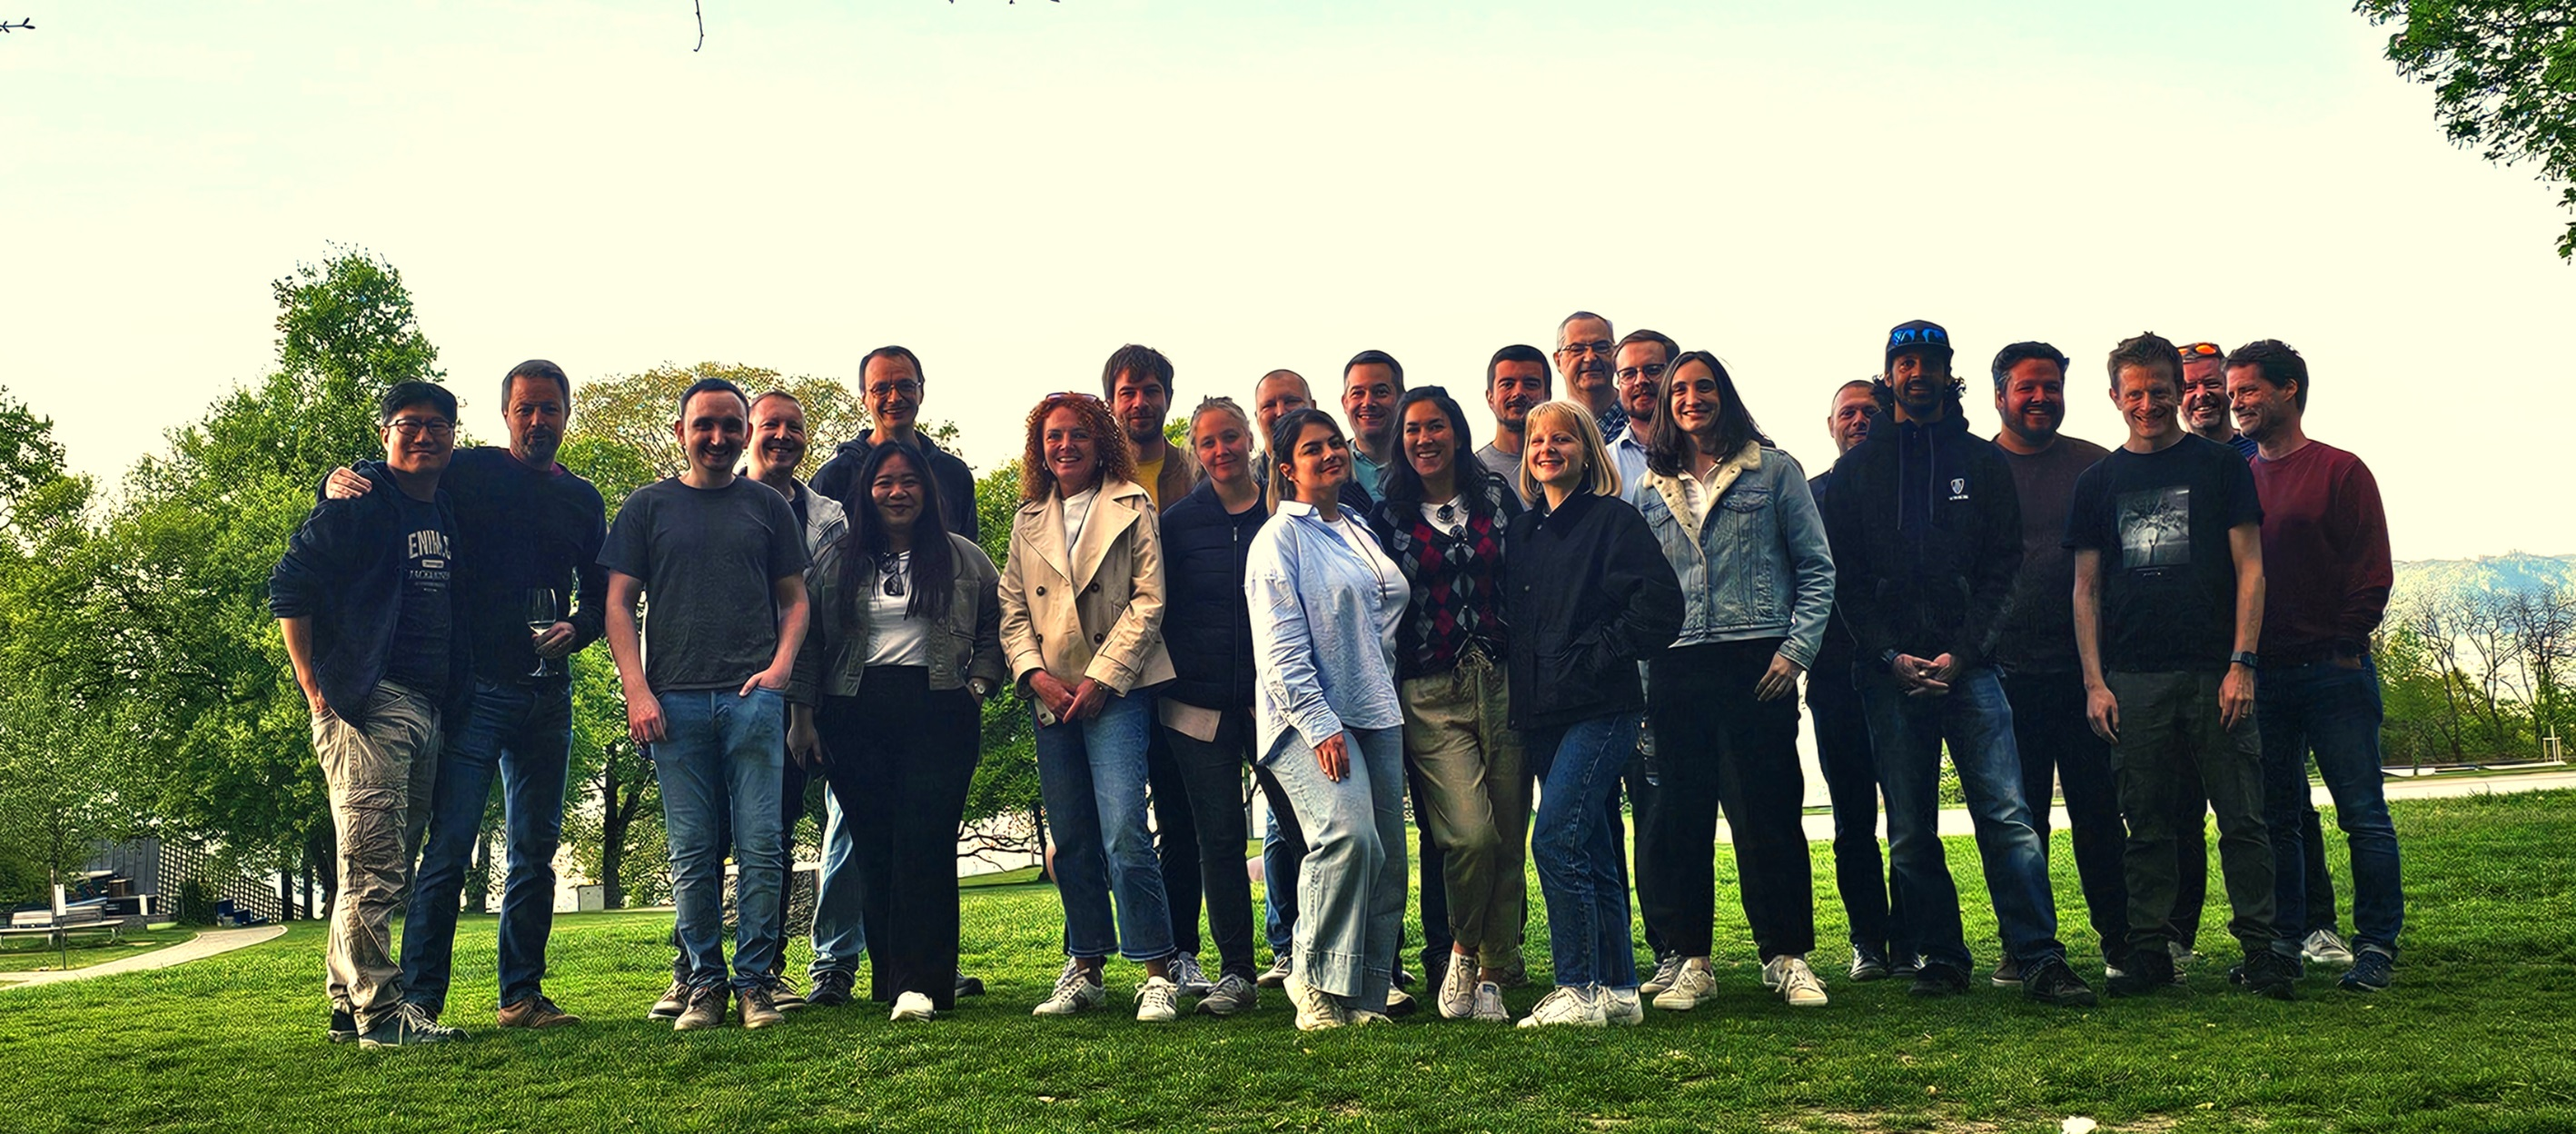
\includegraphics[width=0.8\textwidth]{./content/img/ProjectManagement/BizDevOps_Team.png}
    \caption{Picture of DWH LS OPS team}
    \label{fig:dwhlsops_apero}
\end{figure}


Within the Swiss Post this team is also referred as a \textbf{Busi}ness \textbf{Dev}elopment \textbf{Op}eration\textbf{s} (\gls{BizDevOps})  team, because it contains all required personnel, to create, deploy and maintain reporting solutions. This starts with \gls{businessanalyst}s to evaluate existing reports and their usage, and to document and specify them for further updates or re-engineering. This continues through the implementation, which is carried out first by data engineers and then by business intelligence (\gls{BI}) engineers. Finally, the business side is involved in testing these reports and also serves as the main source when it comes to questions of how or what to implement. Due to the size of this team and the different responsibilities, the DWH LS OPS team consists of three separate sub-teams. These teams are ordered along the process of postal services as introduced in the full mail piece lifecycle being: Receiving, Sorting, Transport, Customs clearance (German acronym is \gls{ASTV}), \textbf{D}elivery \textbf{\&} \textbf{F}inance (\gls{DandF}), and finally the planning focused Parcel Volume Planning and Forecasting (german acronym is \gls{MPP}).

\begin{figure}[H]
    \centering
    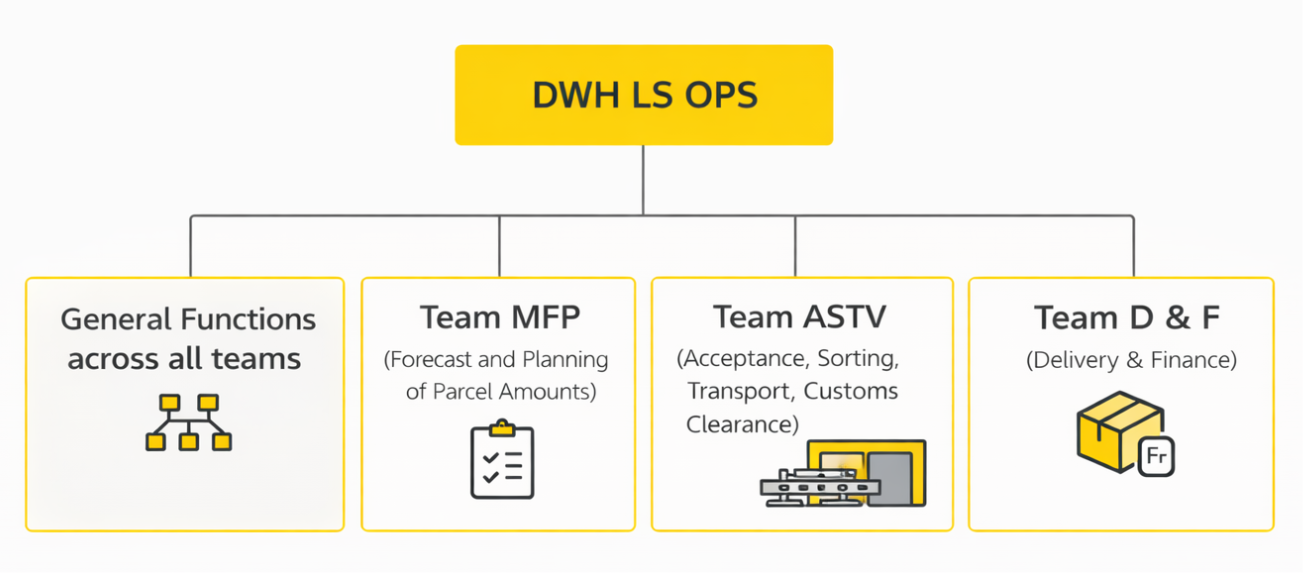
\includegraphics[width=0.8\textwidth]{./content/img/ProjectManagement/BizDevOps_OrgChart.png}
    \caption{Team and sub-team organisation}
    \label{fig:dwhlsops_member_names}
\end{figure}

\subsubsection*{AWS modernisation team}
\label{sec:AWSmodernisationteam}
Swiss Post is currently in a process the modernisation of the AWS cloud environment, which the Swiss Post itself describes as follows:

\textit{Swiss Post is currently pursuing a strategic modernisation of its AWS-based data lake with the objective of improving developer efficiency, increasing operational reliability, and establishing a modern, data-driven architecture. According to internal documentation, the initiative is aligned with defined key performance indicators and aims for completion by the end of the first quarter of 2026 \cite{SwissPostAWSModernization}.}

This modernisation is performed with the assistance of consultants as part of improving AWS usage in DWH LS OPS. The improvements are detailed in 15 \gls{KPI}s across topics such as \gls{AWSGlue} job optimisation and deployment pipeline improvements. With the assistance of the consultants, best practices are applied to the development of \gls{ETL}, as well as general improvements to deployment pipelines. Most importantly for this project, the initiative also includes \gls{DQM} improvements. As a reference, a screenshot of the Confluence landing page describing the initiative is shown below:

\begin{figure}[H]
    \centering
    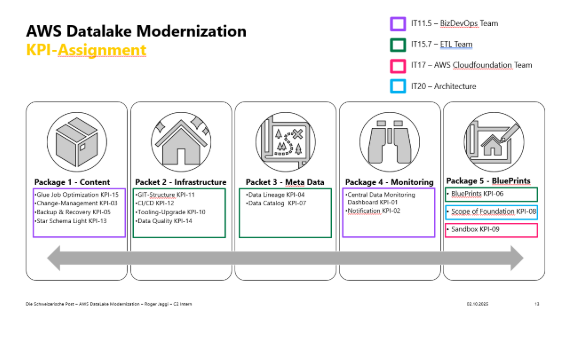
\includegraphics[width=0.8\textwidth]{./content/img/ProjectManagement/AWS_Modernisation_StartPage.png}
    \caption{The start page of the AWS modernisation, listing KPI and latest news}
    \label{fig:aws_modernisation_startpage}
\end{figure}

This team consists mainly of consultants with long-term experience in assisting companies in becoming proficient with AWS. They support data engineers at Swiss Post by improving existing code and reviewing it for potential enhancements. This is relevant for Swiss Post, as the development of the cloud infrastructure started without full architectural support and therefore has room for improvement.

\begin{figure}[H]
    \centering
    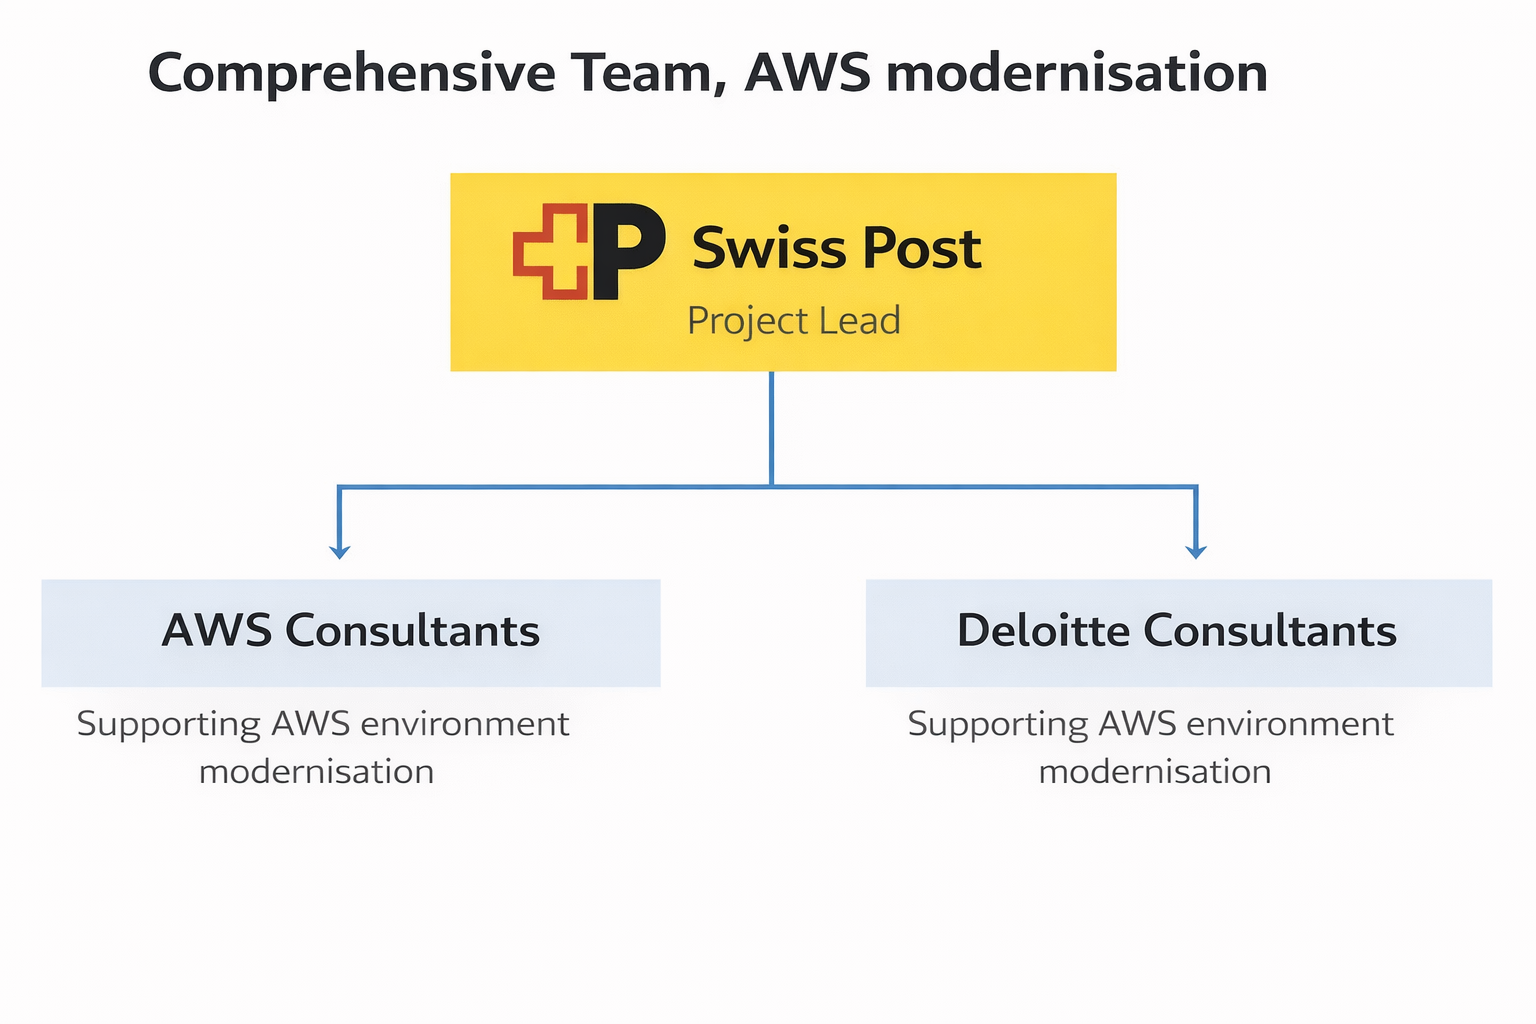
\includegraphics[width=0.8\textwidth]{./content/img/ProjectManagement/AWS_Modernisation_Setup.png}
    \caption{The team setup of the AWS modernisation}
    \label{fig:aws_modernisation_teammembers}
\end{figure}

\subsubsection*{DQM team}
\label{sec:DQMteam}
The third team relevant to the project is the \gls{DQM} team. The team serves KPI 14 Data Quality within the AWS modernisation. Their goal is described on Confluence as follows: specify, review, and implement an MVP to enable data scientists and ETL engineers to forward data quality measures to a monitoring dashboard for both business users and developers.

\begin{figure}[H]
    \centering
    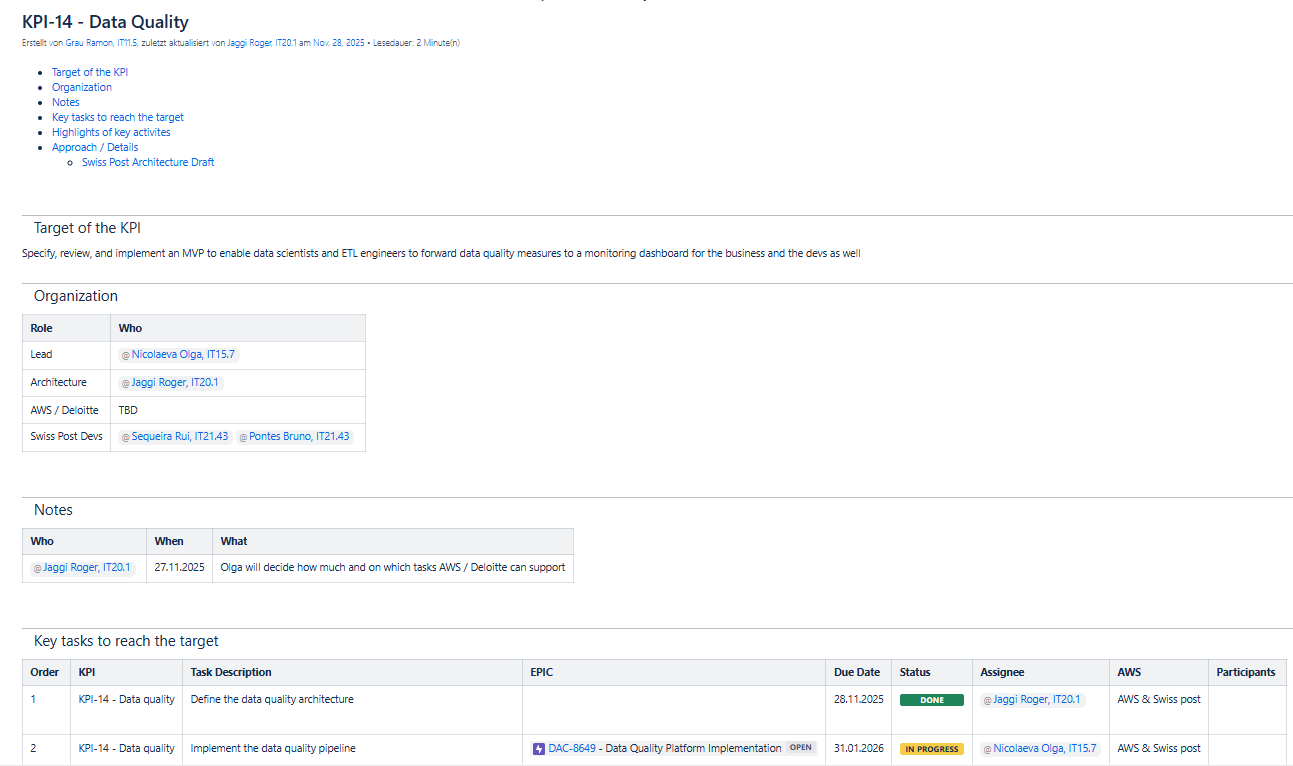
\includegraphics[width=0.8\textwidth]{./content/img/ProjectManagement/Startpage_DQM_KPI14.png}
    \caption{The KPI 14 Data Quality start page on DWH LS OPS Confluence}
    \label{fig:dwhlsops_kpi14_dqm}
\end{figure}

The team consists of three developers with the assistance of a lead data engineer. This setup ensures that the developers can deliver results efficiently, while the lead data engineer provides design guidance and solution structure.

\begin{figure}[H]
    \centering
    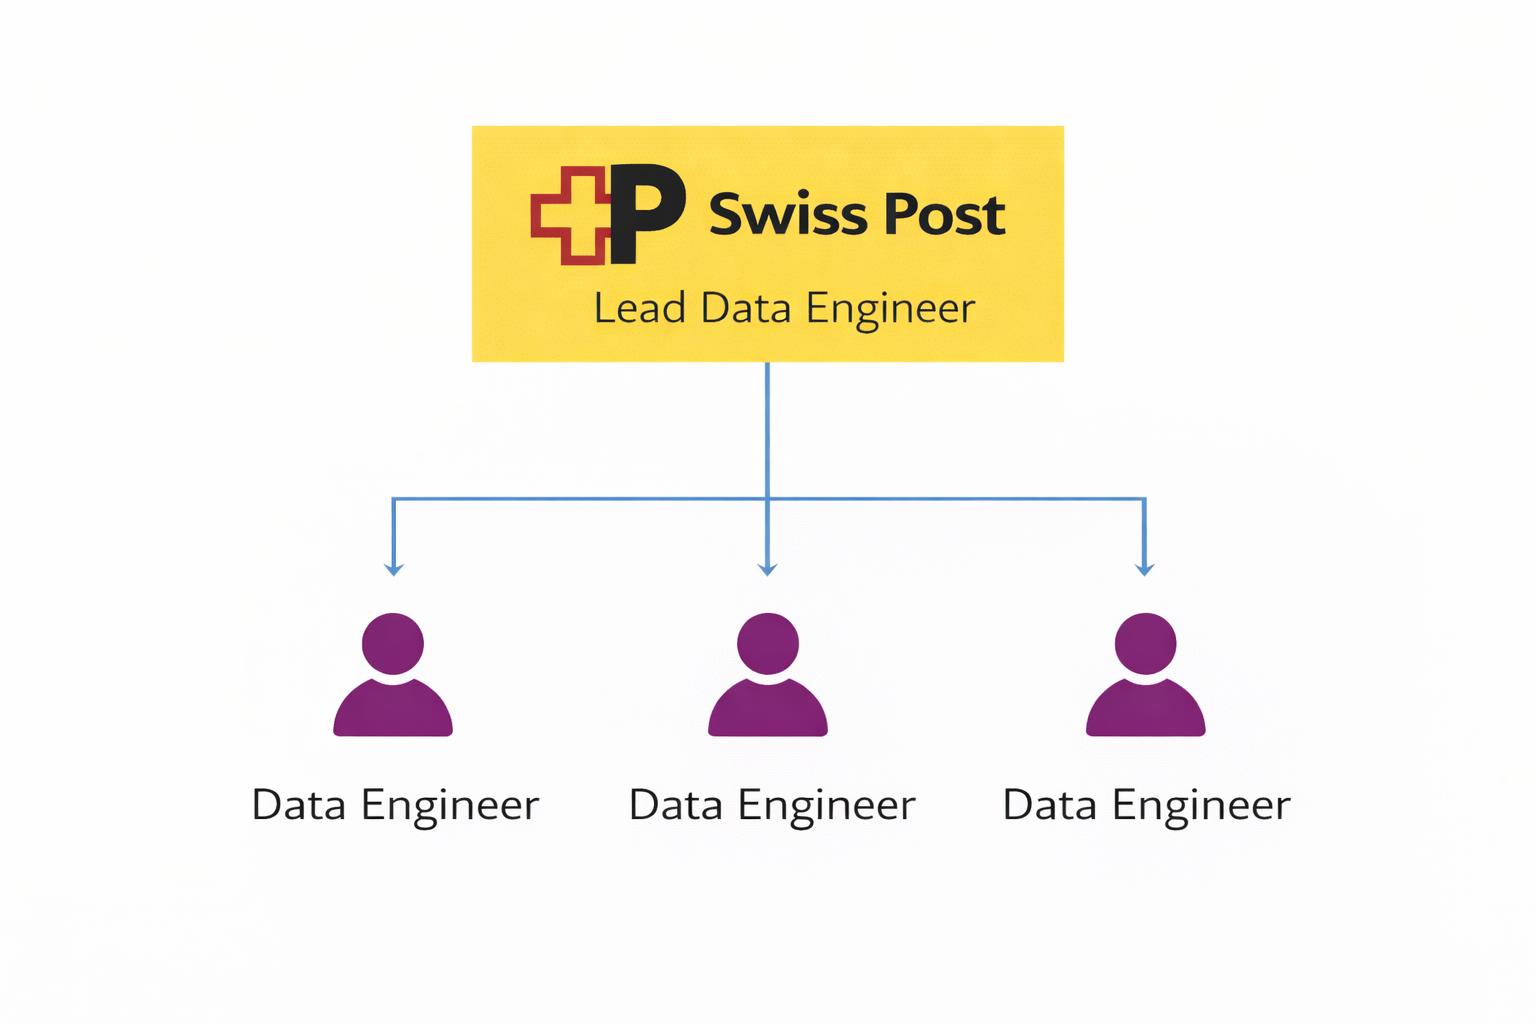
\includegraphics[width=0.8\textwidth]{./content/img/ProjectManagement/DQM_KPI14_Team_NoNames.png}
    \caption{The DQM team setup}
    \label{fig:dwhlsops_kpi14_team_dqm}
\end{figure}

\subsection*{Academic project team}
\label{sec:AcademicTeam}
The academic team consists of the author and the academic advisor. The author conducts the practical work, which includes analysis, implementation, and evaluation. The advisor provides expertise in the academic process and acts as a sparring partner regarding the writing process and project management, offering methodological and academic supervision.

\begin{figure}[H]
    \centering
    
\includegraphics[width=0.8\textwidth]{./content/img/ProjectManagement/ProjectTeam_clean.png}
    \caption{The academic team setup}
    \label{fig:academic_team}
\end{figure}



\section{Project management methodologies}
\label{ProjMgmtMethods}
This section details how the different teams manage themselves. This is done for reasons of transparency, so that the reader understands which project management methods the individual teams use. This highlights an additional level of complexity in the working environment. Not all teams are addressed in every subsection, as the project team was not involved in all teams’ methods to the same depth. First, project management methods are highlighted, followed by the different timeline management approaches. In the following figure, the different boards and management methods are aligned around the central academic team to illustrate the broad set of methods.


\begin{figure}[H]
    \centering
    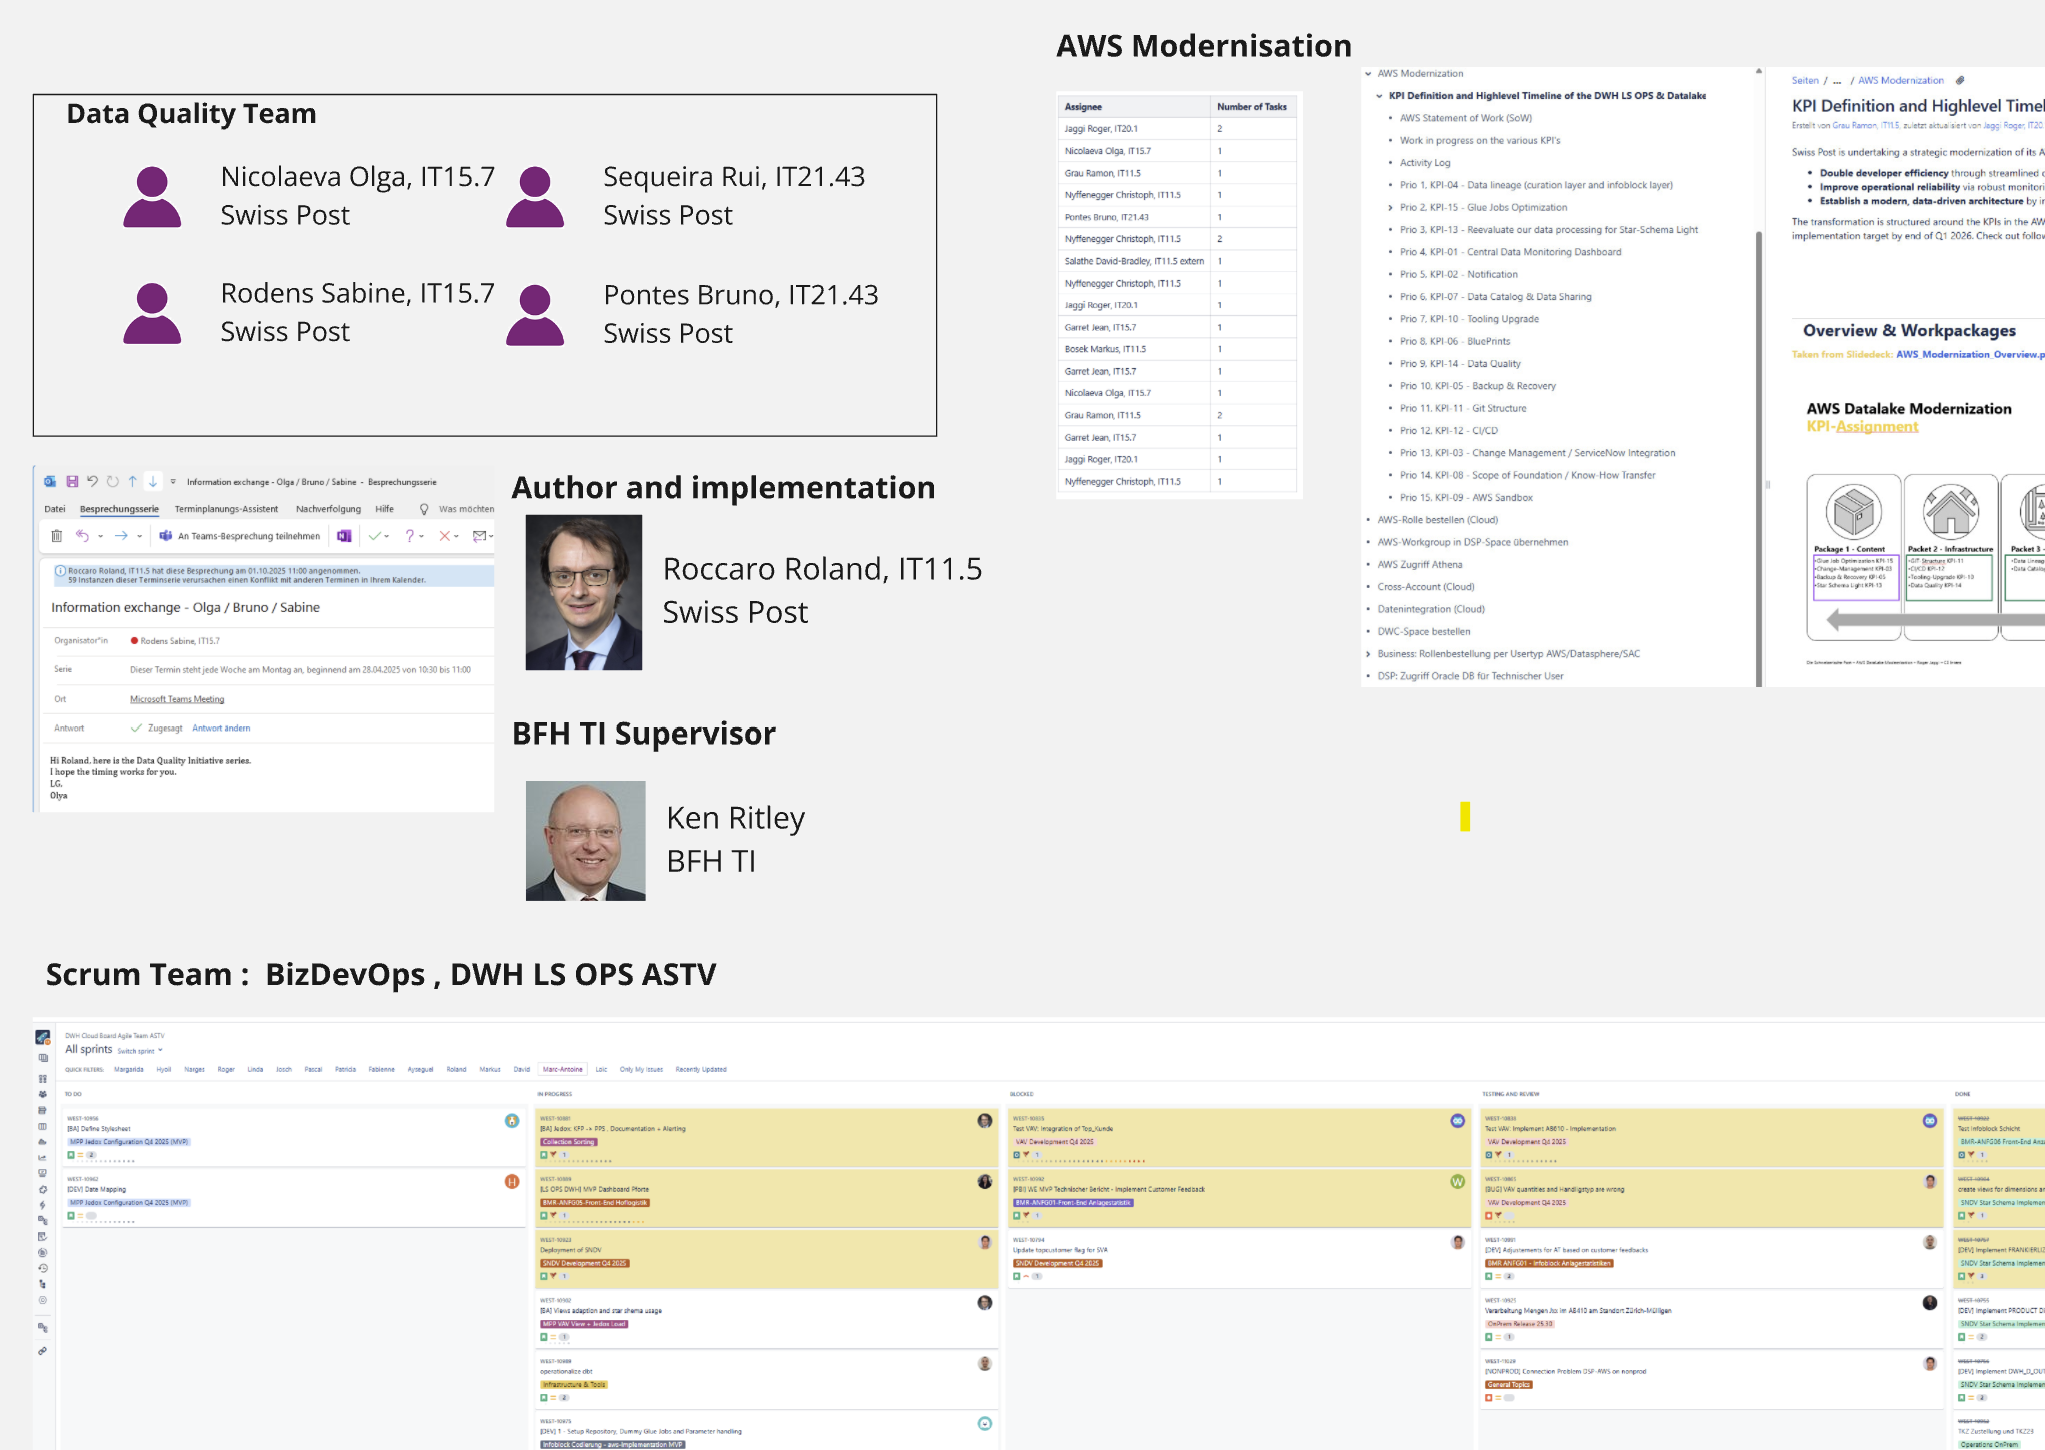
\includegraphics[width=0.8\textwidth]{./content/img/PostTeams_Tools.png}
    \caption{All methods shown in one figure. Top left: DQM team with weekly meetings. Top right: AWS modernisation using a Confluence page. Bottom: DWH LS OPS and academic team using Jira.}
    \label{fig:projmgmt_methods_one_pic}
\end{figure}


\subsection*{Project management}
Project management for this project consists of two main elements. These are Scrum and weekly meetings.

\subsubsection*{Scrum}
The \gls{DWHLSOPS} team is organised as a \gls{BizDevOps} \gls{scrum} team (see Section \ref{sec:DWHLSOPSTeam}). The AWS modernisation teams join these Scrum teams (see section \ref{sec:AWSmodernisationteam}). The full set of rituals defined for Scrum is used, including daily meetings, sprint retrospectives, sprint planning held every two weeks, and reviews held every four weeks. In addition, a weekly Scrum meeting is held to maintain communication between the ASTV, D\&F, and MPP teams. The meetings are shown in the first screenshot, while the second illustrates a noteworthy team definition: the rules of engagement established for collaboration, which are a result of the retrospectives.


\begin{figure}[H]
    \centering
    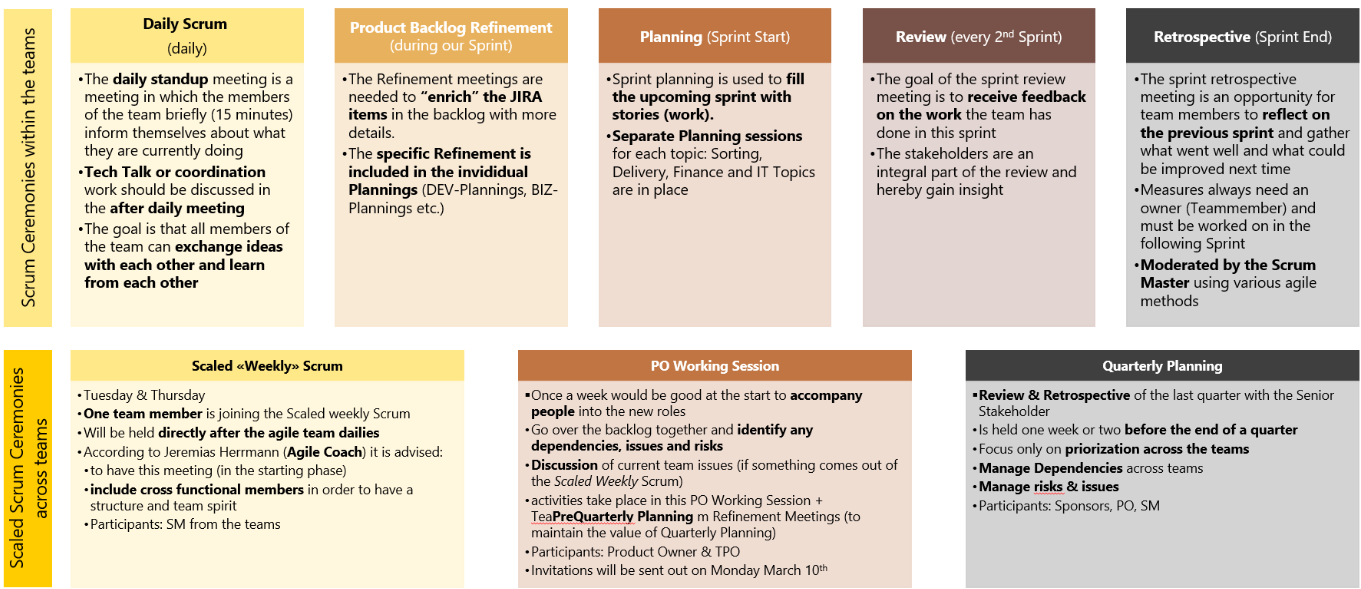
\includegraphics[width=0.8\textwidth]{./content/img/ProjectManagement/BizDevOps_ScrumCeremonies.PNG}
    \caption{Scrum ceremonies of DWH LS OPS  BizDevOps team}
    \label{fig:projmgmt_bizdevops_scrumMeetings}
\end{figure}

\begin{figure}[H]
    \centering
    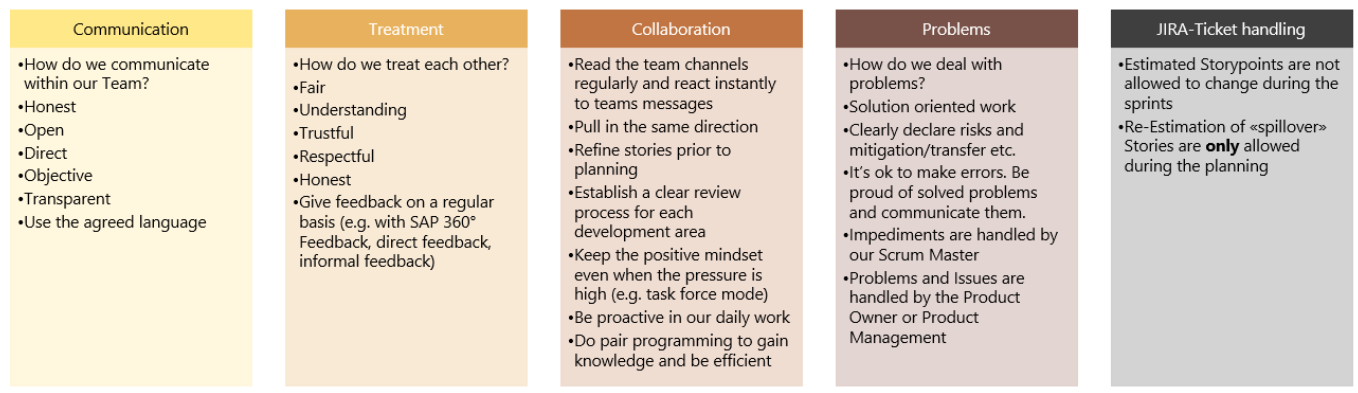
\includegraphics[width=0.8\textwidth]{./content/img/ProjectManagement/BizDevOps_RulesOfEngagement.png}
    \caption{Rules of engagement of DWH LS OPS  BizDevOps team}
    \label{fig:projmgmt_bizdevops_rulesofengagement}
\end{figure}

\subsubsection*{Weekly Meetings}
Contact with the \gls{DQM} team is handled through weekly meetings (see section \ref{sec:DQMteam}). These serve as minimal update sessions during which weekly progress is communicated to all team members. While the developers in the DQM team are themselves also part of a Scrum team, their sprint management is out of scope.

\subsubsection{Adapted Scrum}

The project team handles task planning and progress management using Scrum, however, in an adapted fashion. The DWH LS OPS board is used for a dual purpose. As a result, the sprint lengths are also two weeks. The board is linked to the shared Miro board for easier management within the academic team. The Scrum events are mainly held within the DWH LS OPS team. The academic team, however, performs a separate planning confirmation every two weeks and retrospectives, which happen less frequently. The dates for retrospectives are noted in the Miro calendar.



\subsubsection*{Jour Fixe}

The academic team holds a \gls{JourFixe} every week. This serves to maintain close communication and functions as a check-up meeting. Each meeting follows a defined structure; as an example, the meeting held on 12.10.2026 is described below.

\begin{itemize}
    \item Project check-in and clarification of objectives
    \item Overview of the project and completed deliverables
    \item Current deliverable in progress
    \item Update of initial project description
    \item Status of milestones
    \item Other topics
\end{itemize}

First, a general introduction to the project is provided to serve as a check-in and to allow participants to focus on the project. Second, the deliverables currently being worked on are listed based on the deliverables overview. Third, the status of the milestones is reviewed. Fourth, this is followed by individual agenda items, which can differ from meeting to meeting. In this meeting, these included updates to the initial project description, as well as a check-in regarding open administrative tasks such as handling contracts and payments. Finally, the meeting is closed with an open section in which any other relevant topics may be discussed. These meetings are documented in Miro (see below), structured using a three-block template, and most often recorded using handwritten notes that are later uploaded. Depending on the week's topics, some information, such as the sample below, is added. It shows the question of how to cite sources properly and the options provided.



 \begin{figure}[H]
    \centering
    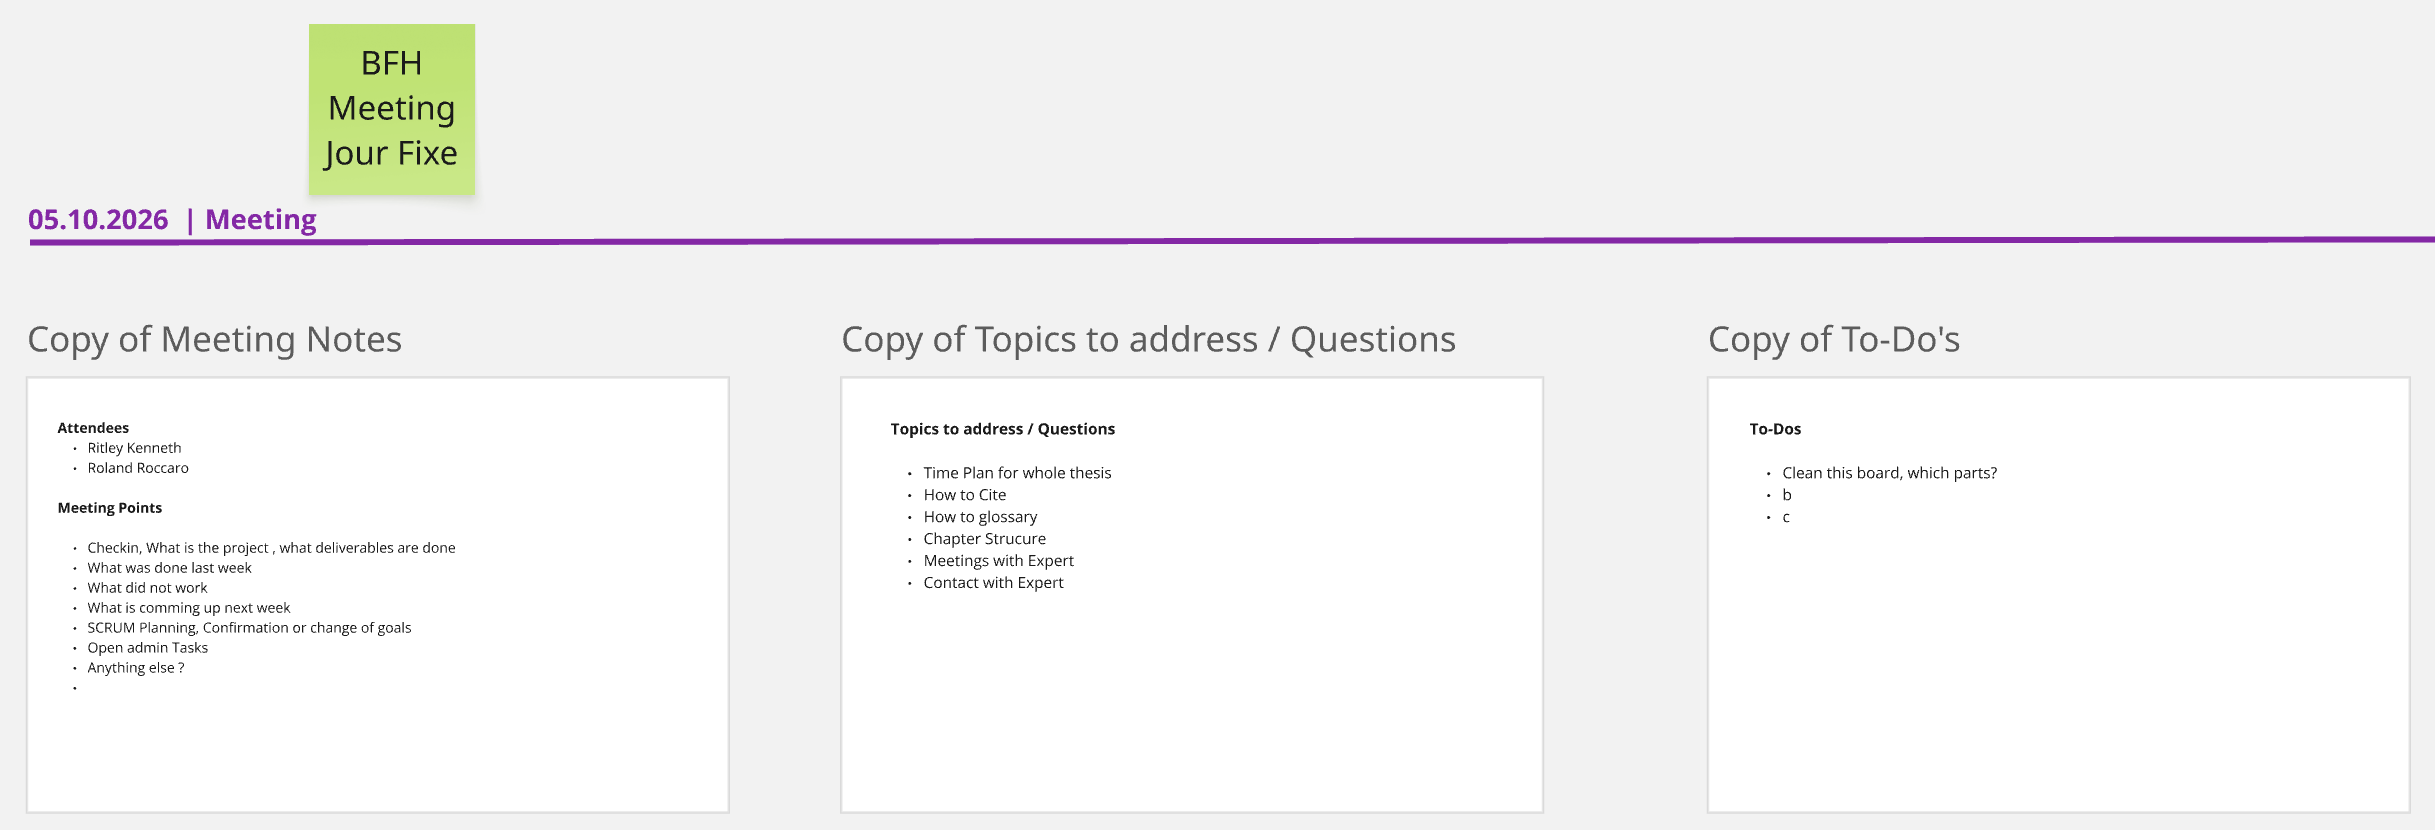
\includegraphics[width=0.8\textwidth]{./content/img/ProjectManagement/Academic_JourFixe.png}
    \caption{Jour Fixe of Academic team, meeting structure and rework}
    \label{fig:jour_fixe_academic_structure}
\end{figure}

\begin{figure}[H]
    \centering
    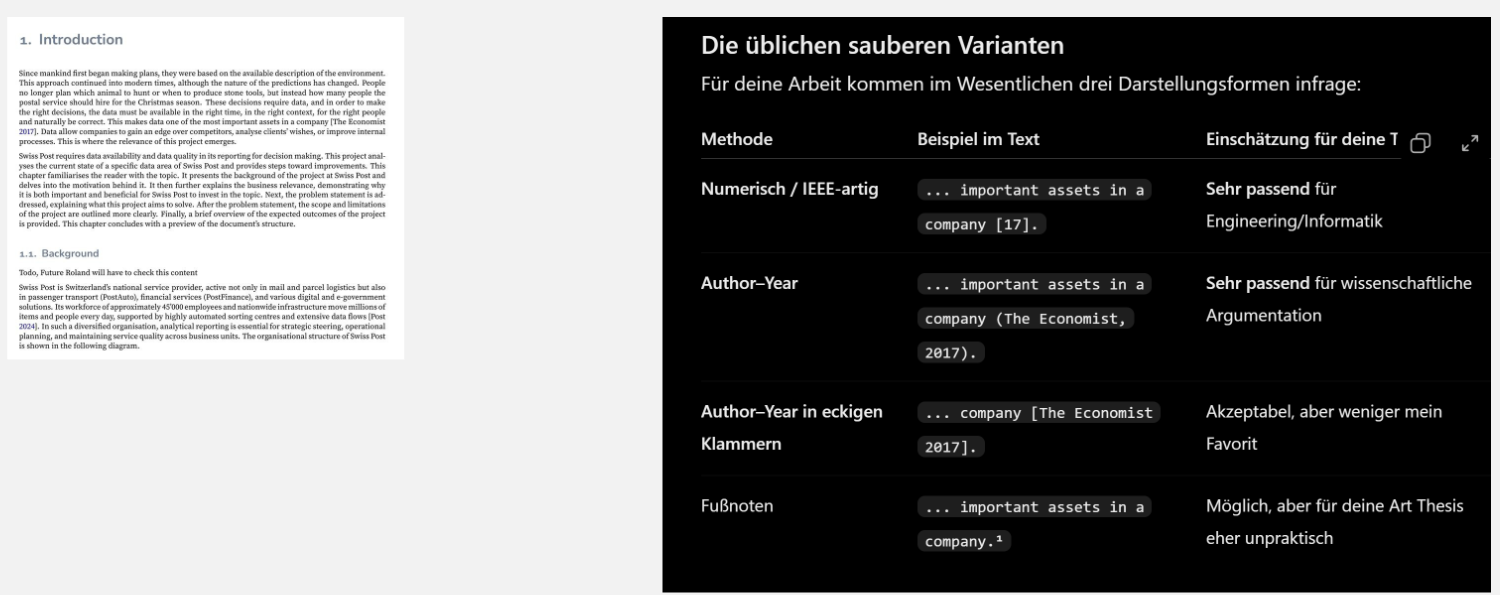
\includegraphics[width=0.8\textwidth]{./content/img/ProjectManagement/Academic_JourFixe_Pre_Notes.png}
    \caption{Jour Fixe documentation of the academic team. Example of a question to be discussed: How should citations be formatted, and is the current citation style appropriate?}
    \label{fig:jour_fixe_notes_academic}
\end{figure}

\subsection*{Timeline management}
Timeline management is performed in different ways by the teams. In this subsection, the planning of actions is described, as well as how staff availability is tracked.

\subsubsection*{Scrum Events}
All teams use Scrum events to manage their weekly progress. Progress on stories is monitored in daily meetings, during which each team member updates the team on progress and issues and indicates whether assistance is needed or deviations from the previously planned approach are required. Sprints encompass the stories the team works on during a two-week cycle. During sprint planning, the stories for the next sprint are defined. The stories added to a sprint represent the commitment the team makes for the sprint, together with the sprint goal. Planning over longer time horizons is conducted through quarterly planning sessions. Every three months, all teams in DWH LS OPS plan which \gls{epic}s should be completed and how many story points should be delivered. These quarterly planning sessions also serve to prioritise epics and allow higher management to introduce priorities.



\subsubsection*{Holidays}
Holidays are noted in the calendars used; this applies to the DWH LS OPS team as well as the academic team. In both cases, every holiday must be recorded with an absence notification. This allows other team members to quickly see whether a team member will be available in the future and to adjust their planning accordingly, or to confirm in daily operations that the person is not available.

\subsubsection*{Phases and milestones}
The academic team also uses phases and milestones to split the work into logical blocks and track its progress over the full duration. The details of these phases and milestones are described in their respective sections.


\section{Tools to support the project management}
\label{ProjMgmtTools}
This section lists the tools used during the project for reasons of transparency. It also allows the reader to evaluate different ways in which these tools can be used. 

\subsection*{Miro}
\label{ProjMgmtToolMiro}
Miro is part of the toolset of both the academic team and the Swiss Post teams. However, in this project, it was used only by the academic team. The reason for using Miro is that it is a lightweight tool that allows combining different data structures on a single board. Miro provides an infinite canvas on which a wide variety of information can be placed. The information can be structured and easily rearranged to regroup related elements. This allows the tool to be used both for early documentation of information and for later restructuring when additional ideas emerge, particularly in the context of long-term documentation. The ability to restructure information visually supports the decomposition and understanding of complex environments.

A full set of screenshots illustrating changes on the Miro board has been moved to the appendix, while the final one is included here (\ref{apendixMiroUsage}). The following screenshot represents the Miro board during the finalisation of the document, zoomed out so that all elements are visible. While this view prevents individual details from being seen, some relevant parts are shown in detail in the following subsubsections.

\begin{figure}[H]
    \centering
    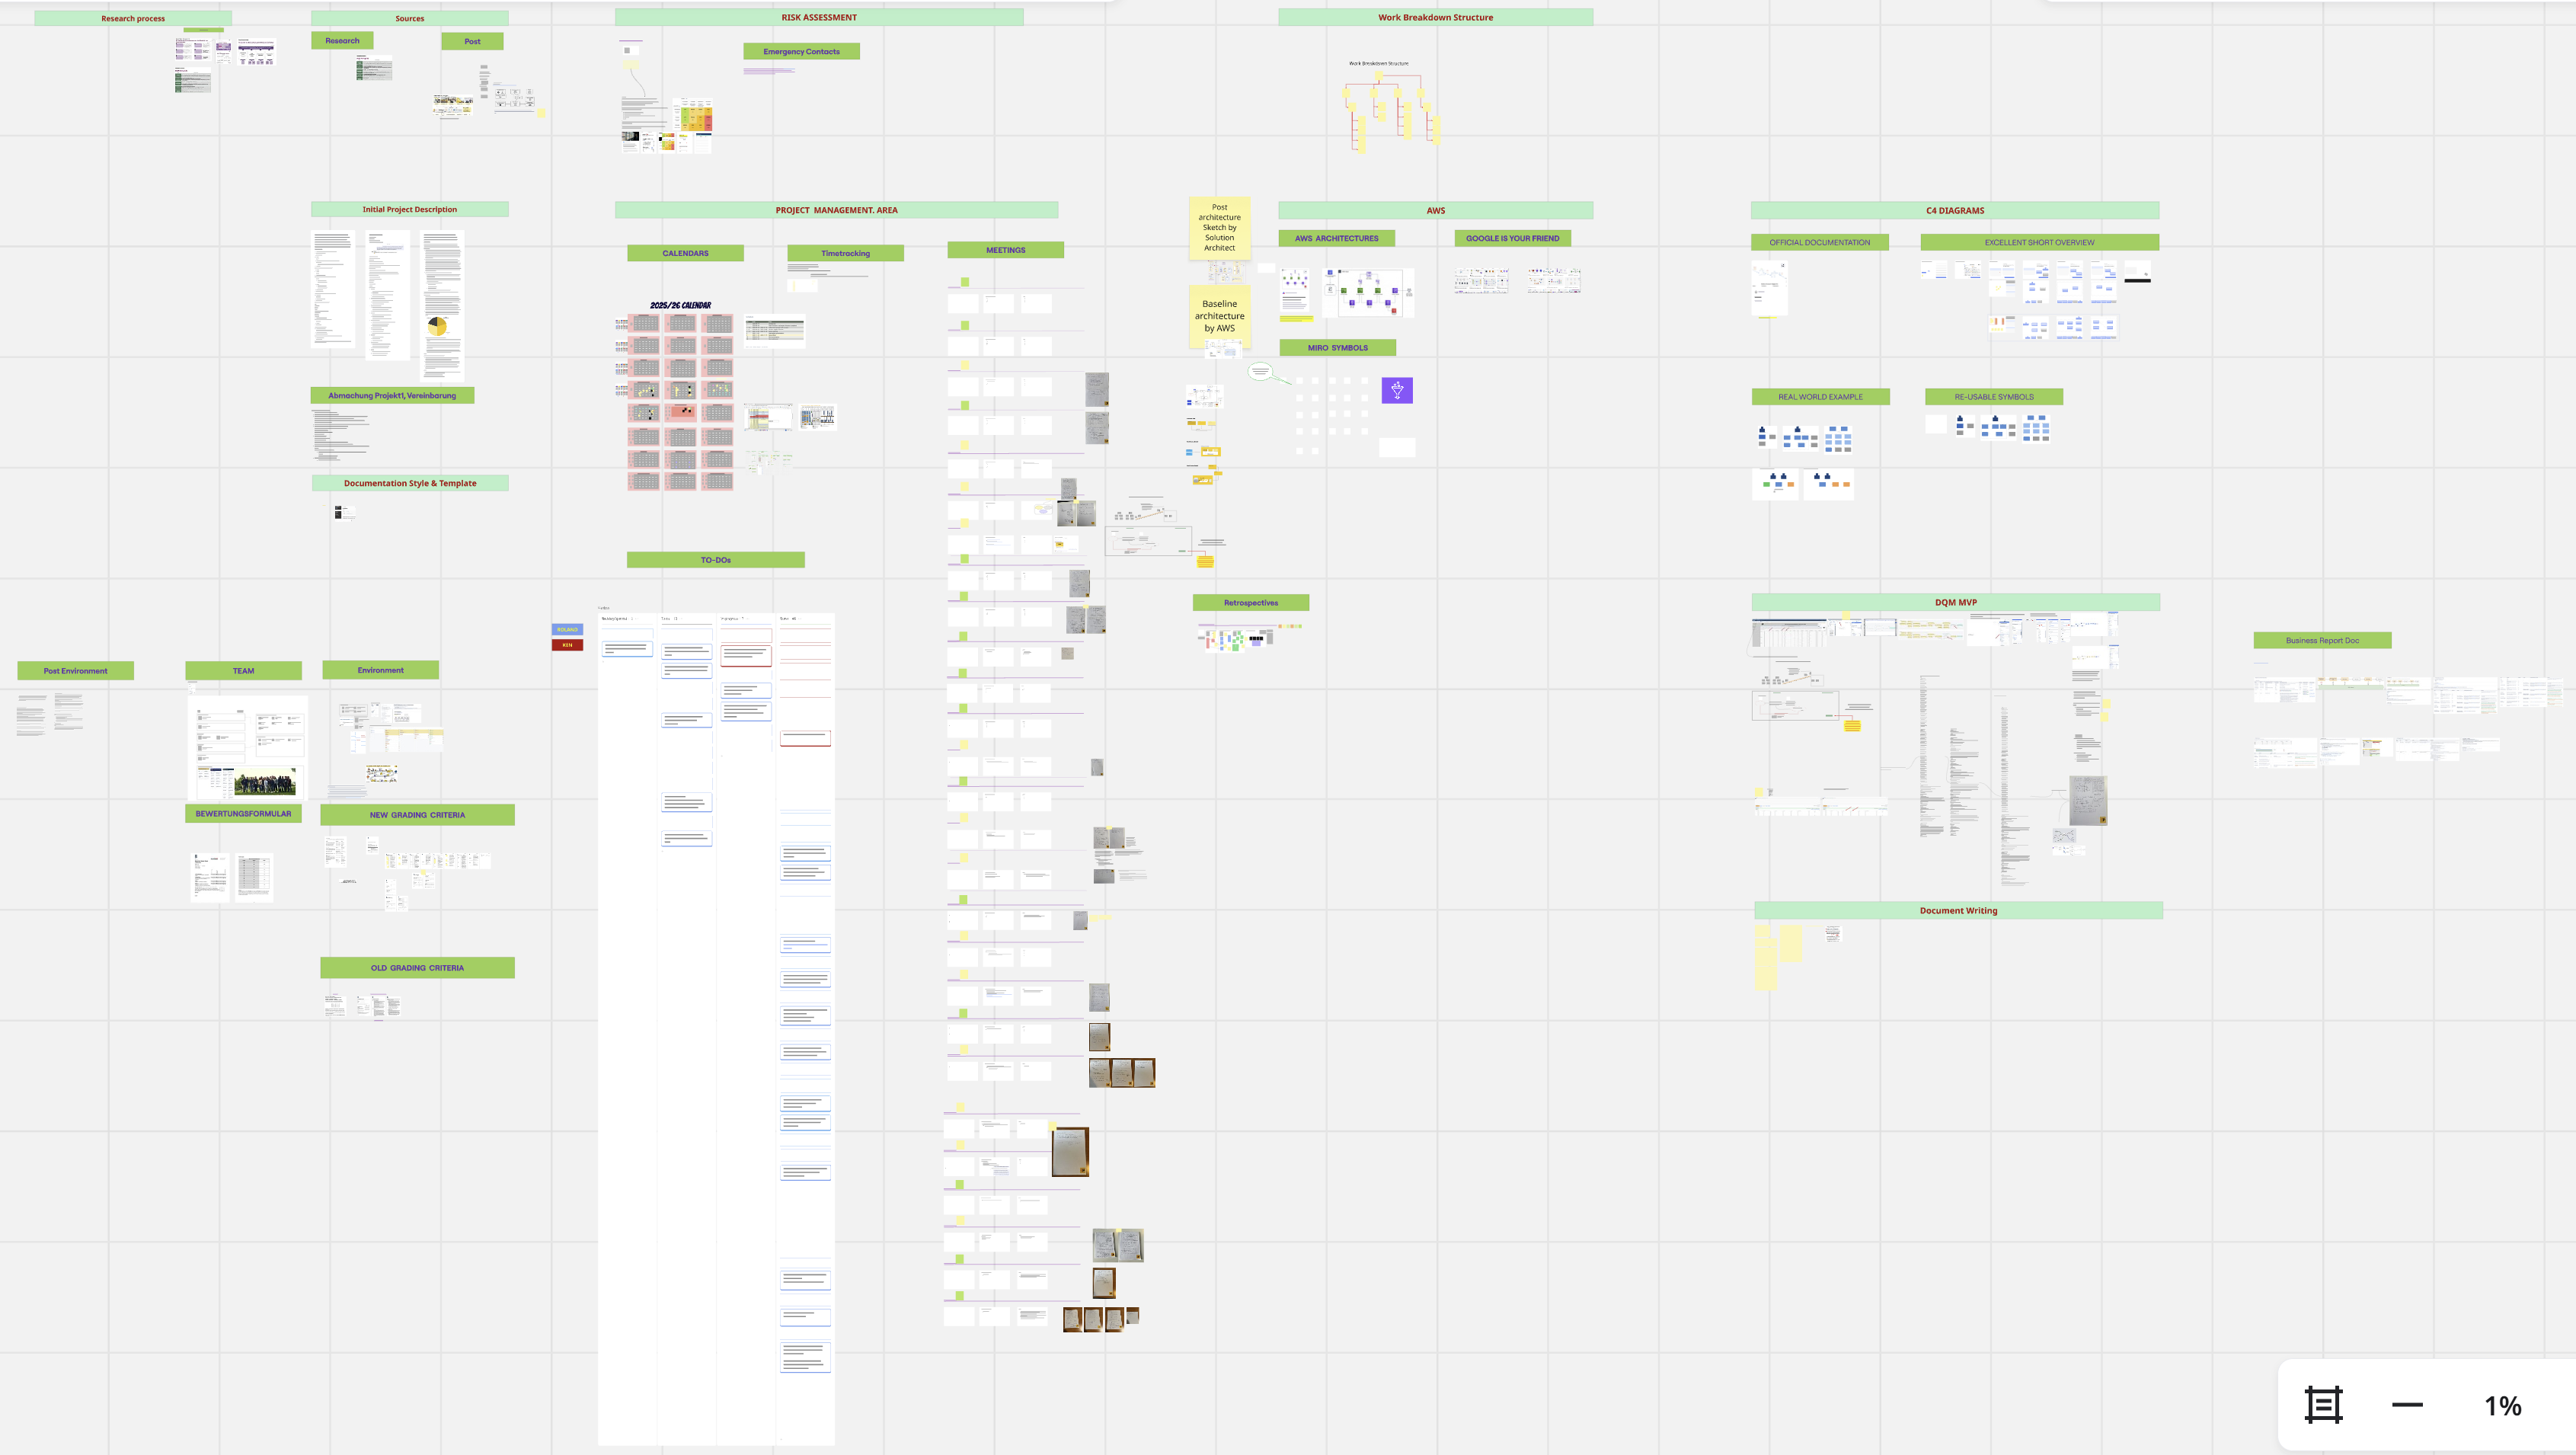
\includegraphics[width=0.8\textwidth]{./content/img/MiroBoard_23-12-2025.png}
    \caption{Miro board documentation, view of 23.12.2025}
    \label{fig:miro_final_board_twentythird_december}
\end{figure}

\subsubsection*{Miro calendar}
The calendar in Miro was primarily used to schedule the milestones. These are shown with green tiles on the corresponding dates, including their number and milestone title. Jour Fixe meetings are marked in yellow whenever they occurred, including adjustments in cases of unavailability. Actual unavailabilities at scheduled Jour Fixe meetings and other times are documented in black. Finally, holidays are marked in teal. In the case of this project, this applied only to the Christmas and New Year holiday period.

\begin{figure}[H]
    \centering
    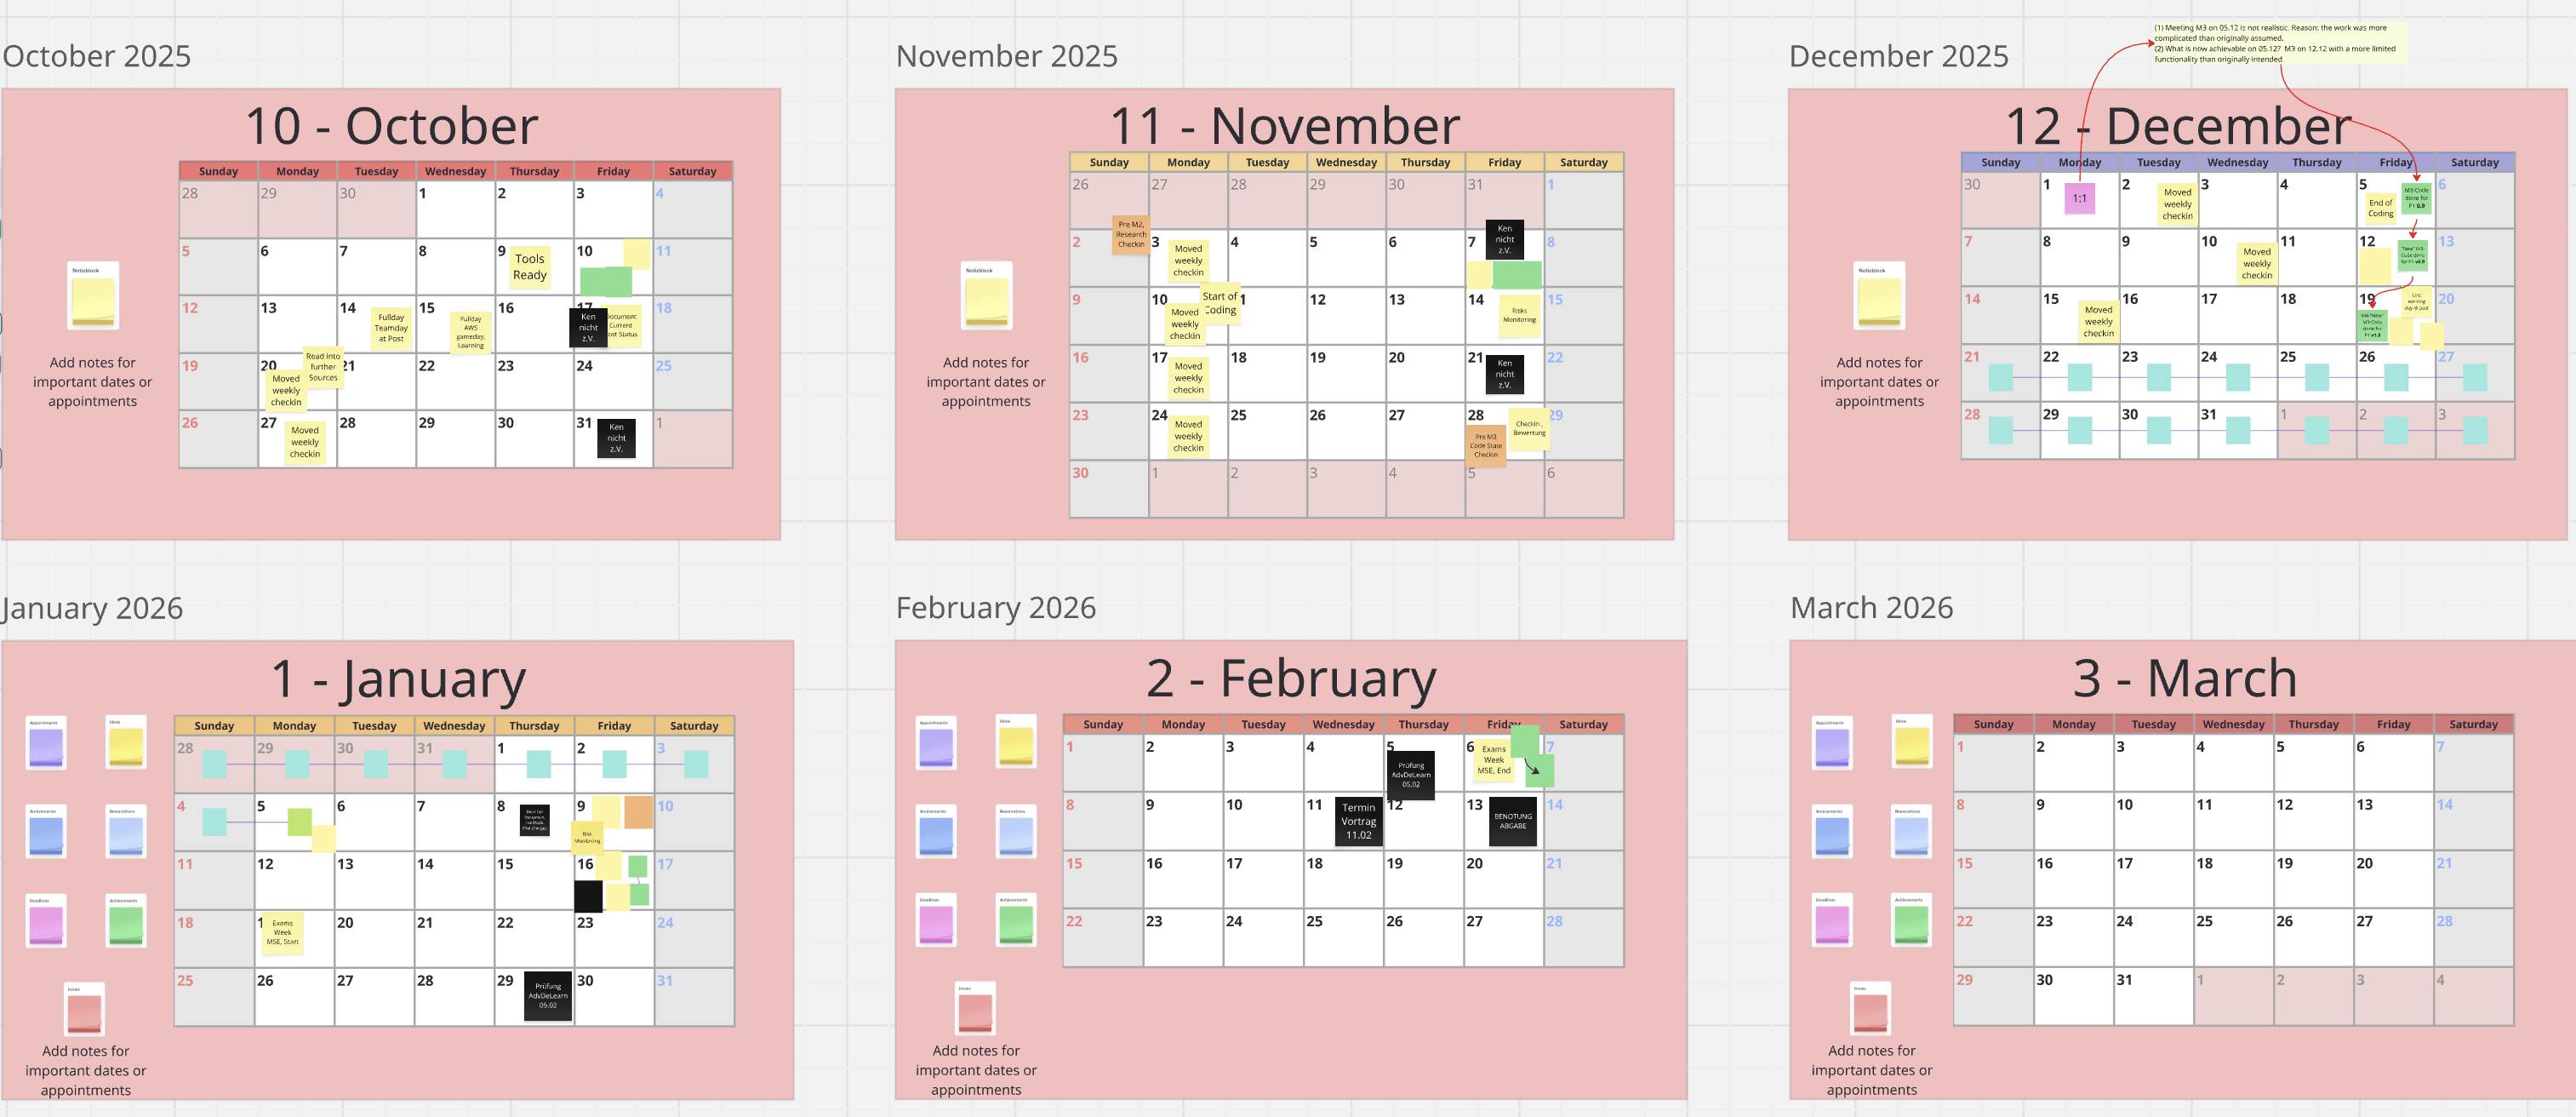
\includegraphics[width=0.8\textwidth]{./content/img/MiroBoard_Calendar.png}
    \caption{Miro board calendar used for coordination and tracking of milestones and related events}
    \label{fig:miro_board_calendar}
\end{figure}

\subsubsection*{Meetings documentation}
The meetings are documented using a layout with three sections, including a coloured tag at the top in yellow for Swiss Post meetings and green for academic ones. From left to right, these sections are structured as follows. First, the meeting points to be discussed are listed; these are copied from the Outlook invitations. Second, the topics addressed are summarised, mostly after the meeting. Third, the to-do block describes any actions that arose during the meeting. Not every meeting includes all sections. Furthermore, meetings are often documented using handwritten minutes. These are uploaded to the right of the meeting blocks without further refinement and serve as references.

\begin{figure}[H]
    \centering
    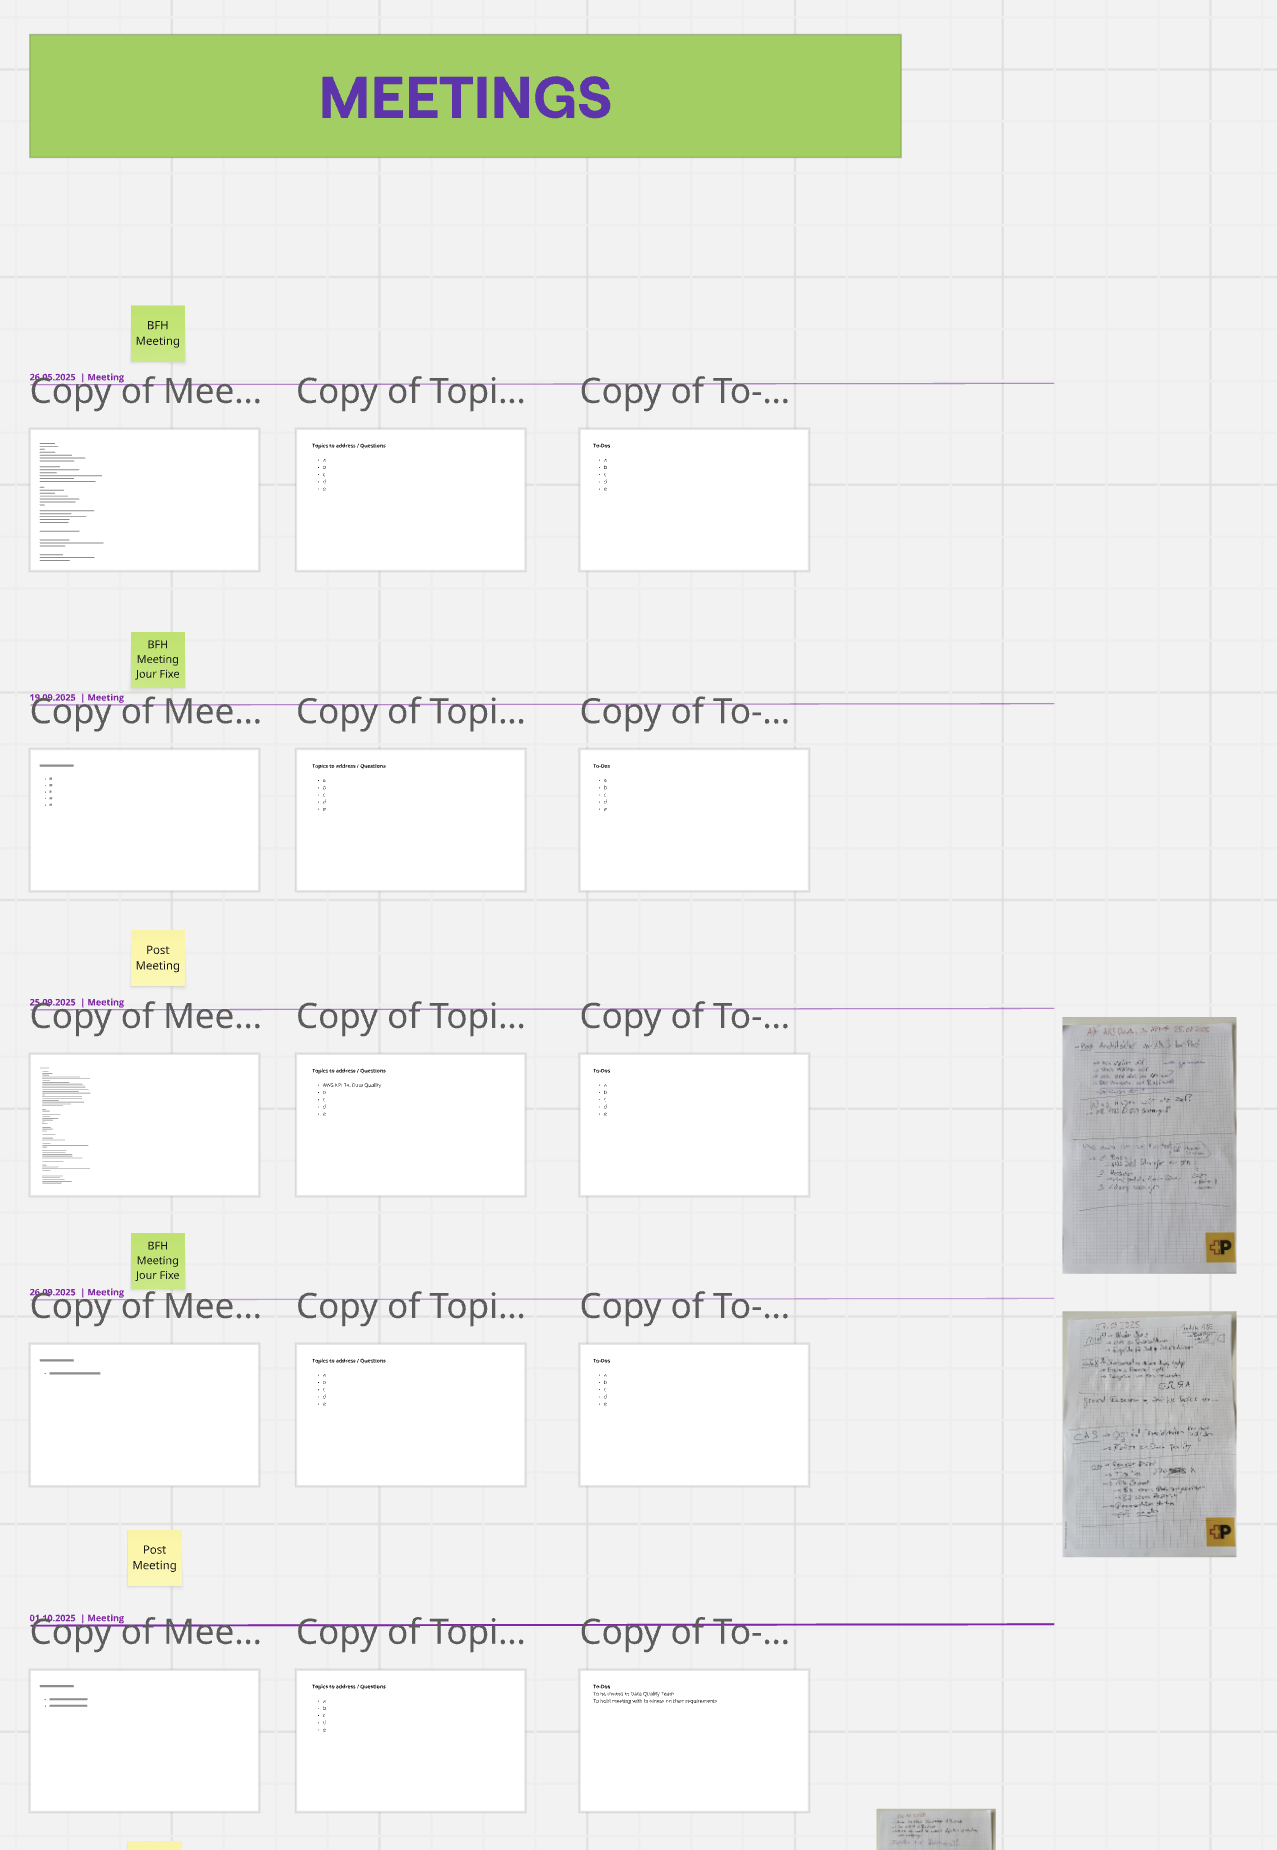
\includegraphics[width=0.8\textwidth]{./content/img/MiroBoard_Meetings.png}
    \caption{Miro board, tracking of meetings: when, who, what}
    \label{fig:miro_board_meetings}
\end{figure}

\subsubsection*{Documentation of the Implementation}
The implementation was first documented in Miro, as the rapid creation of screenshots did not disturb the flow of information gathering. In the following figure, the information-gathering process can be seen, starting from the top left, moving to the right, and then restarting from the left. First, screenshots of the SAC report are shown, followed by navigation towards DSP. Further details on the tools are described in the Implementation chapter.

\begin{figure}[H]
    \centering
    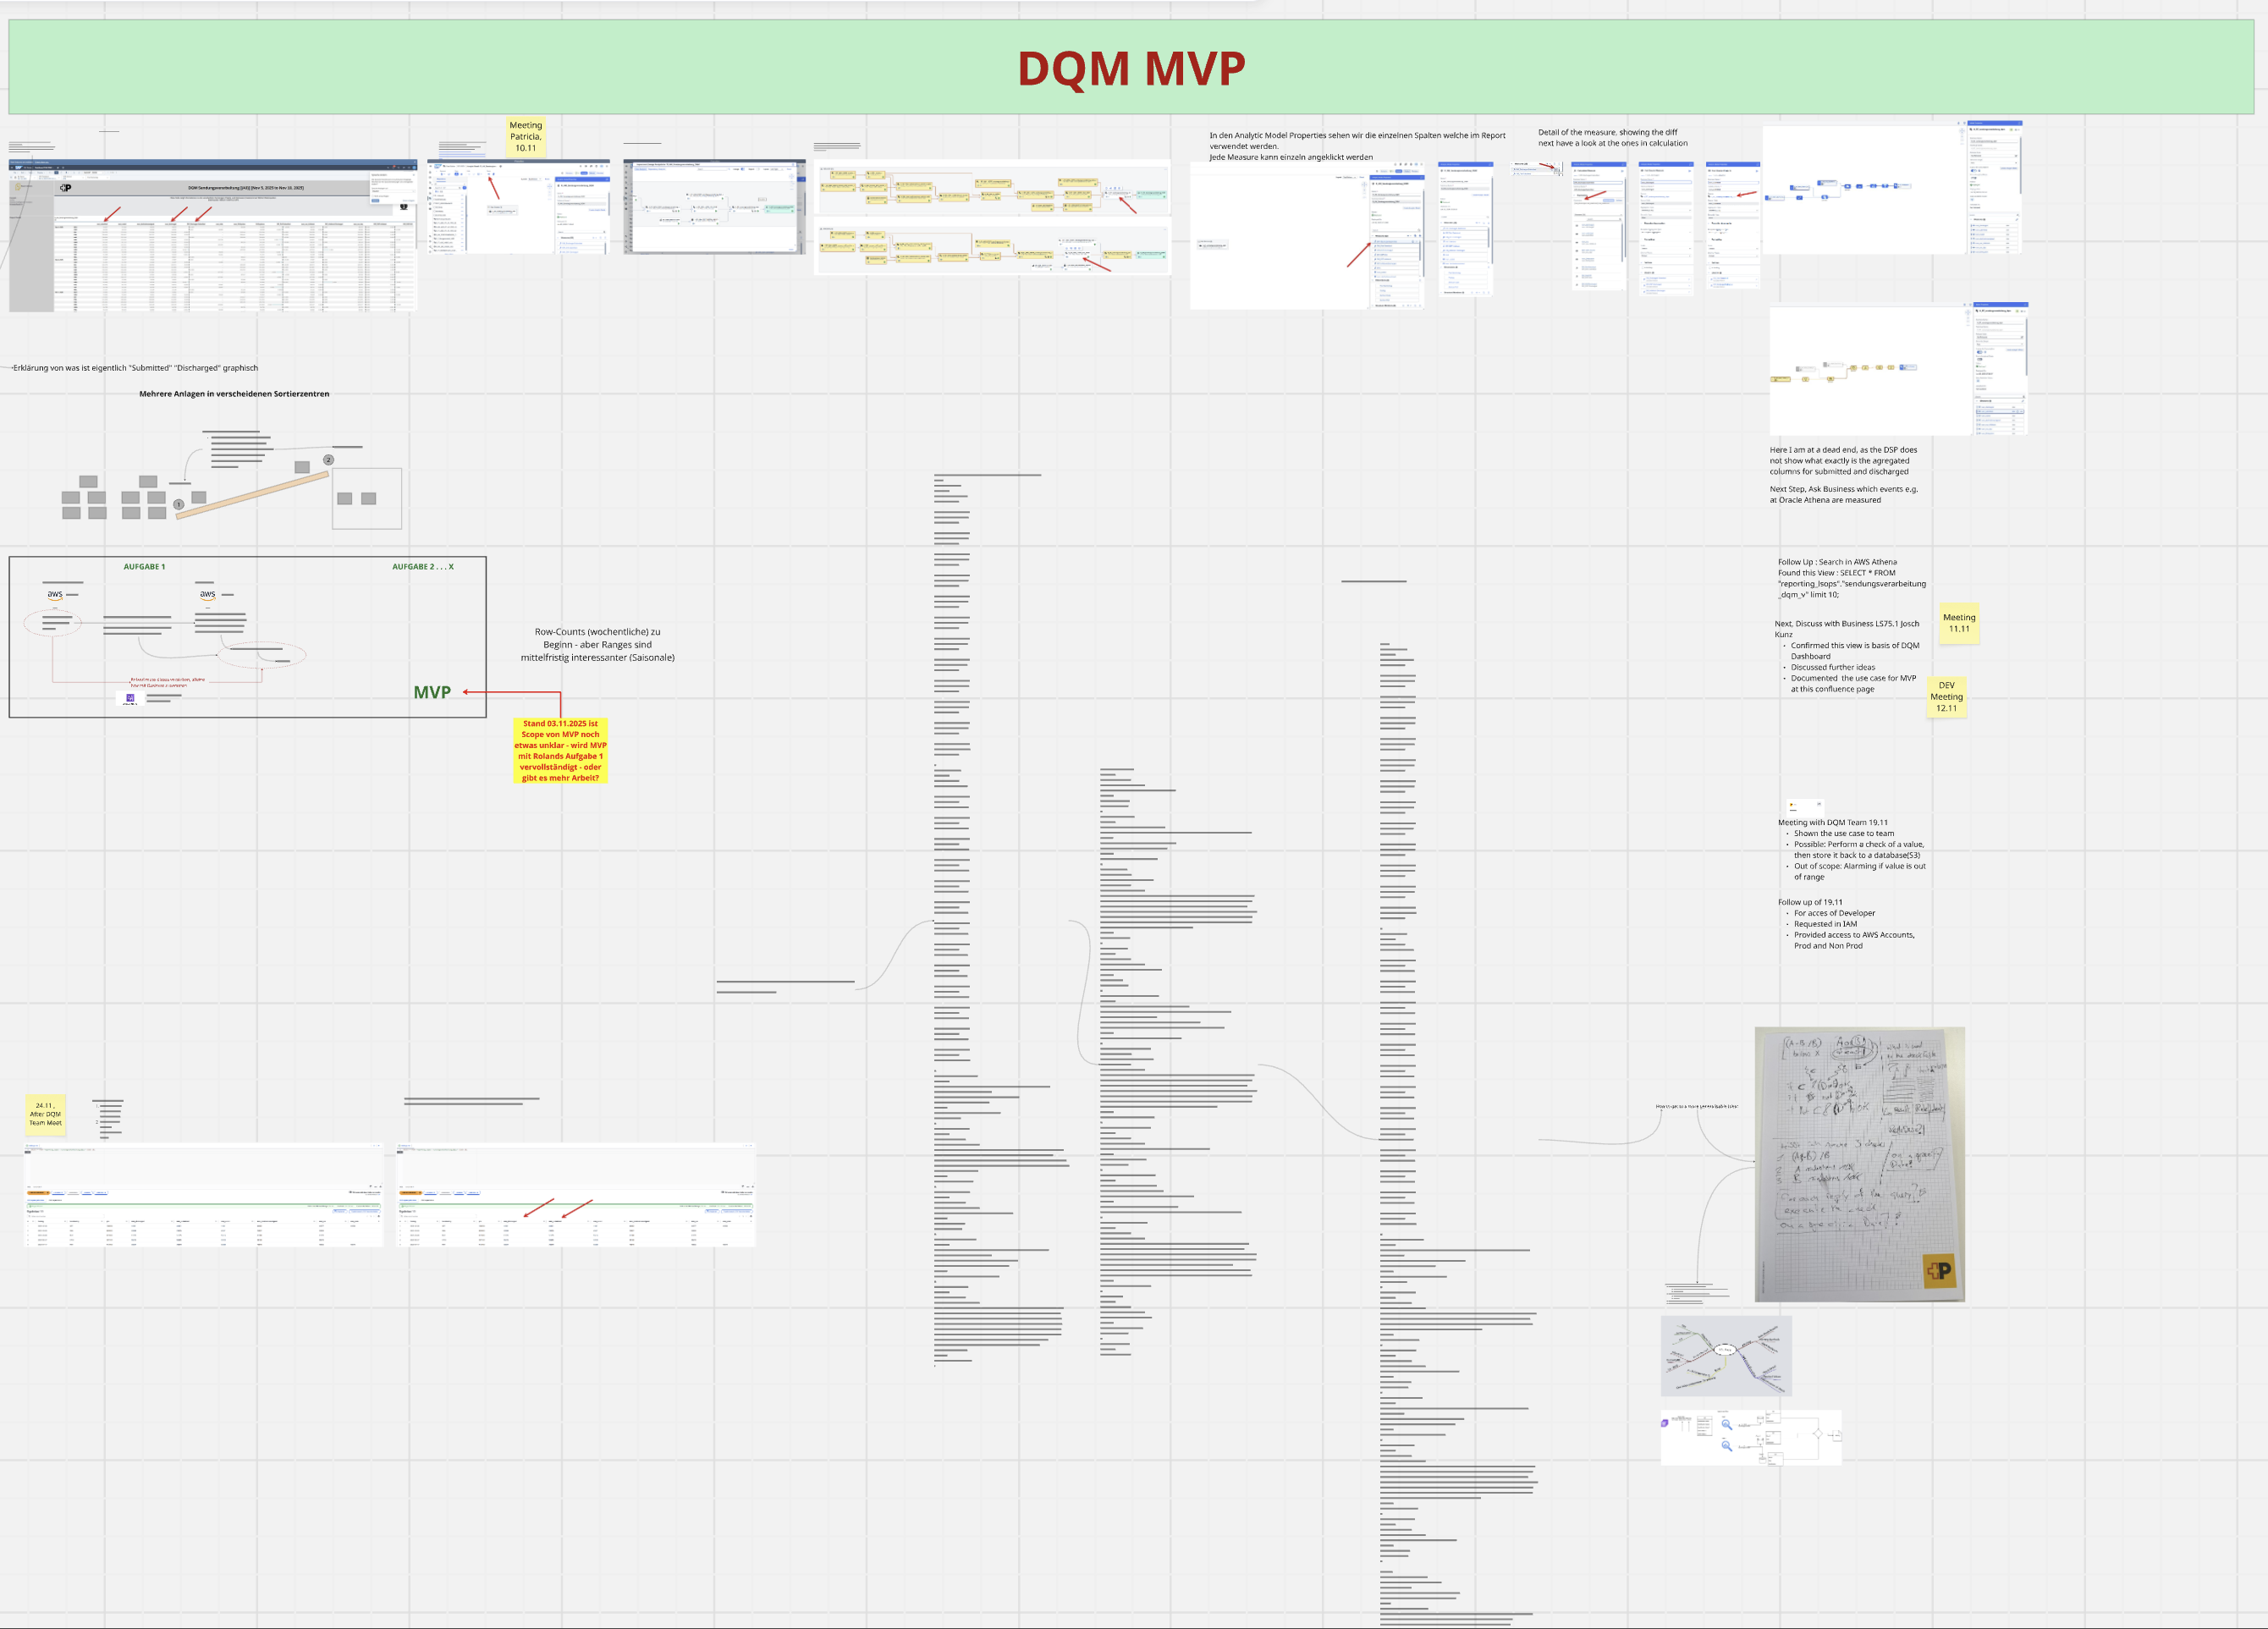
\includegraphics[width=0.8\textwidth]{./content/img/MiroBoard_Implementation.png}
    \caption{Miro board usage for quick documentation during implementation}
    \label{fig:miro_board_implementation}
\end{figure}


\subsection*{Jira and Confluence}

Jira (mainly for issue tracking) and Confluence (mainly for documentation) are both tools provided by Atlassian and are therefore well integrated with each other. The tools are installed on-premises, which limits sharing possibilities outside the Swiss Post network. They are used by the three Swiss Post teams presented in the Teams section. The project team also used Confluence when research results had to be presented as a first use case. While Jira is used for the short-term management of Scrum artefacts, Confluence is used for long-term documentation. An example of such long-term documentation is shown in the following screenshot, illustrating the documentation of a data lineage.

\begin{figure}[H]
    \centering
    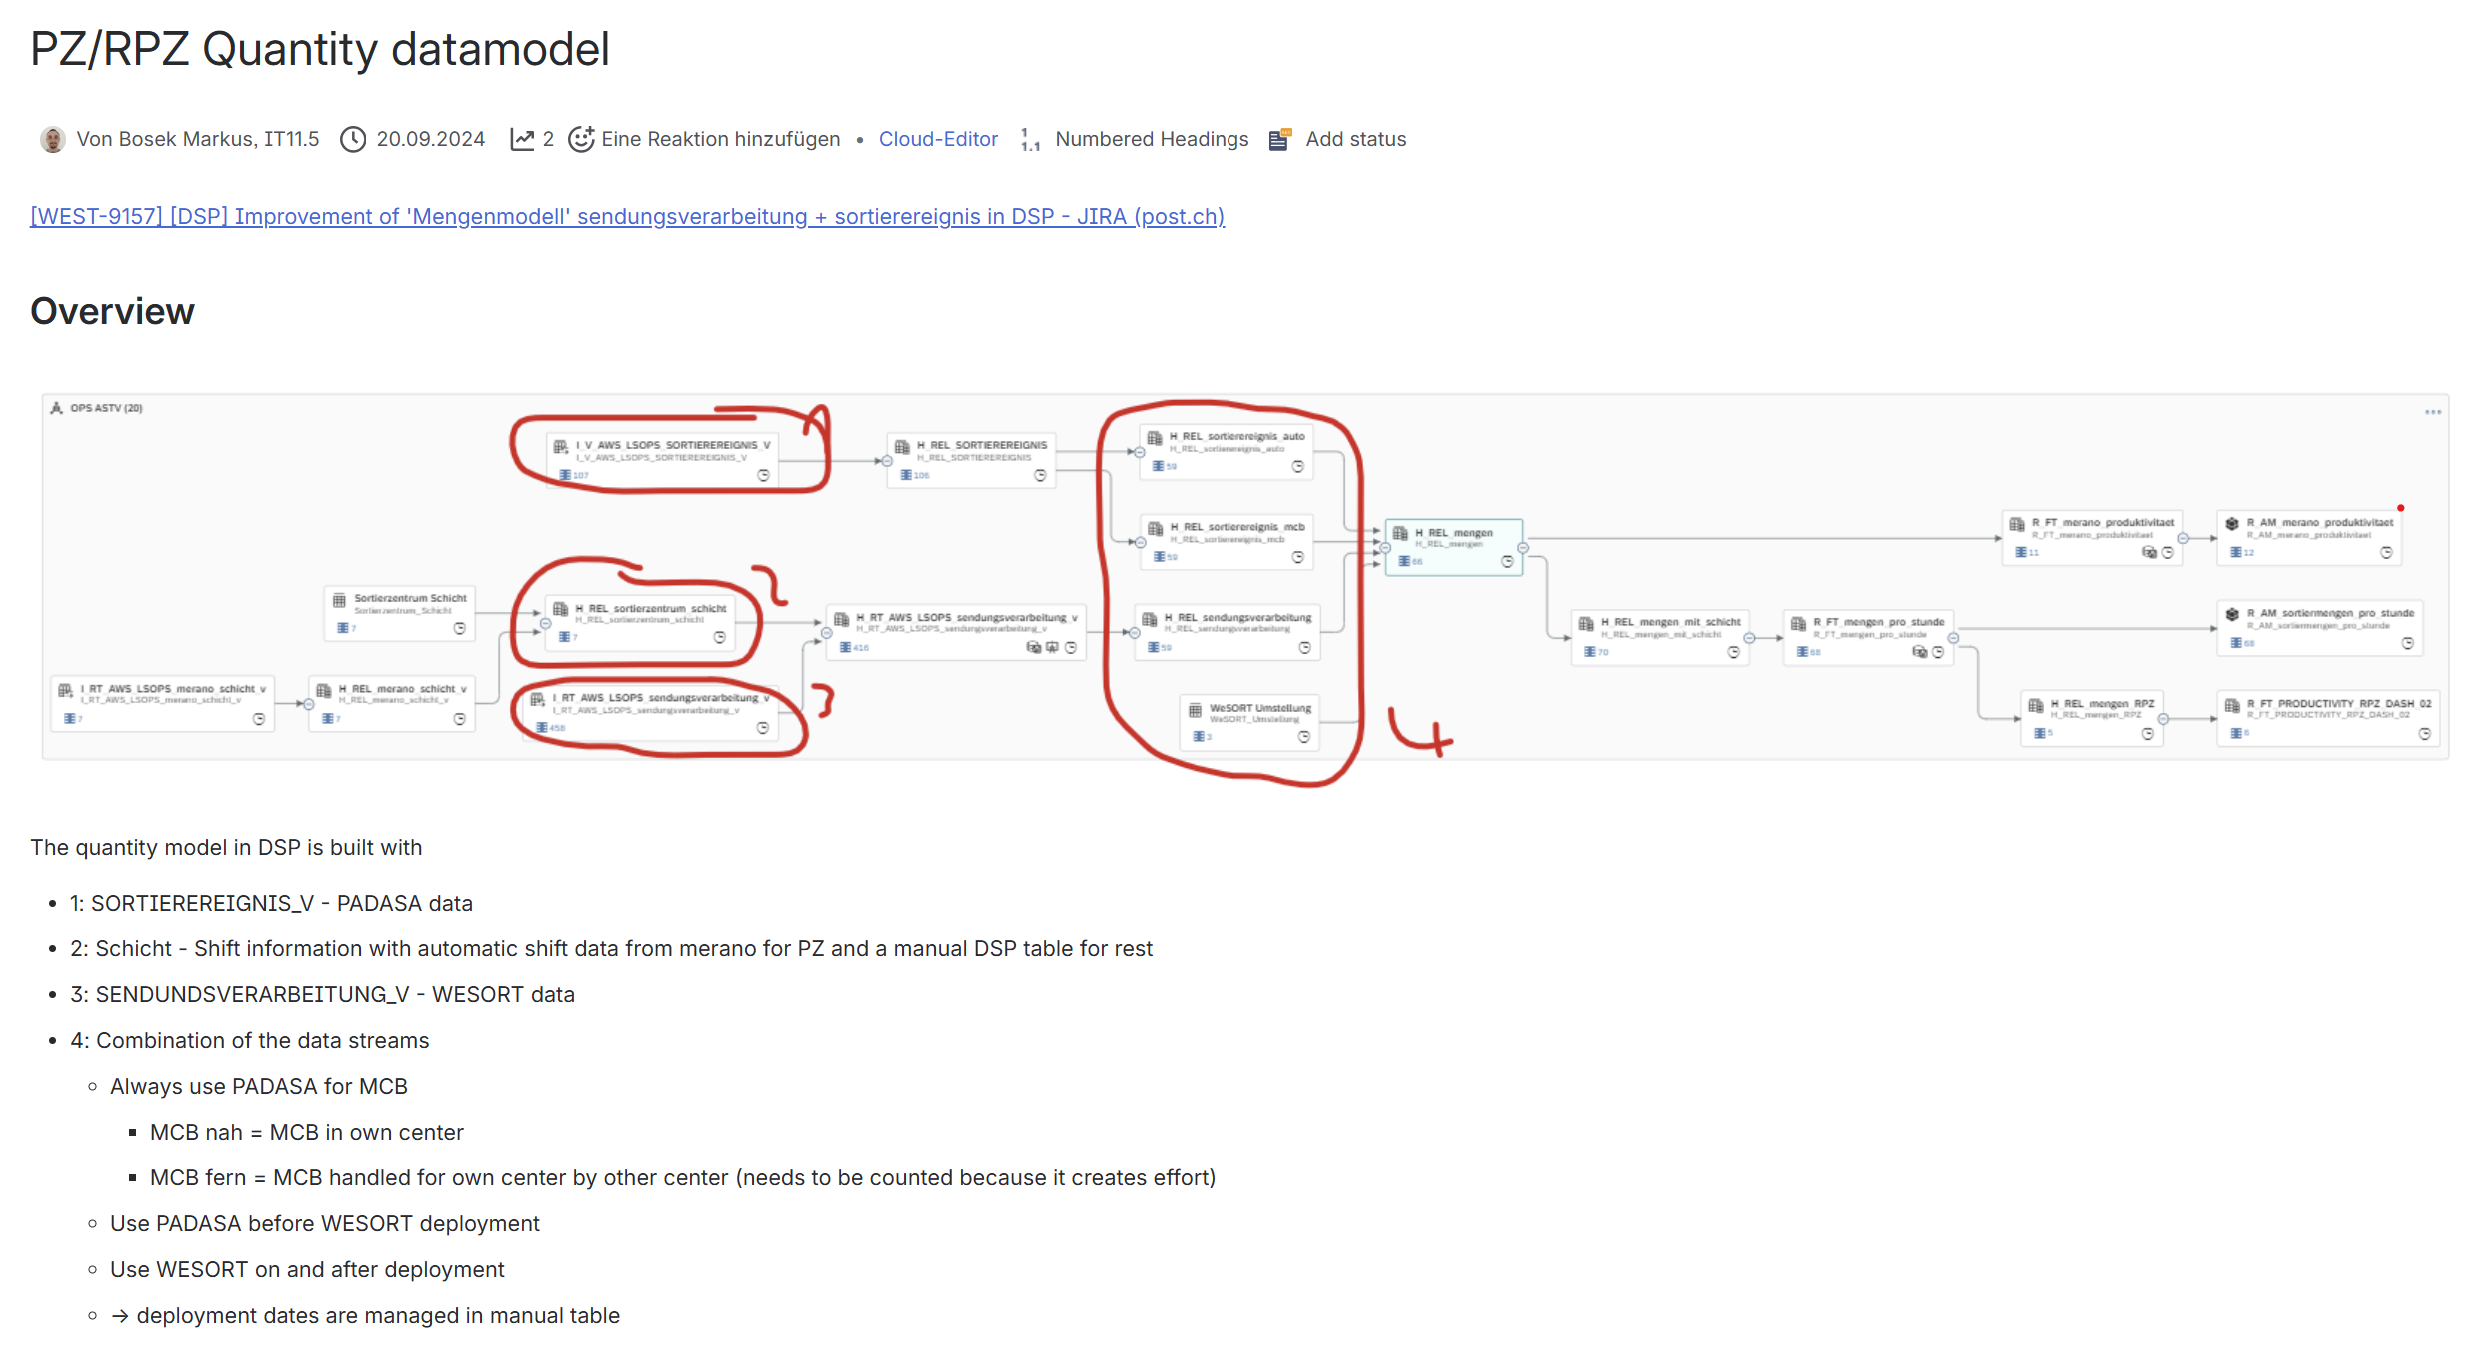
\includegraphics[width=0.95\textwidth]{./content/img/ProjectManagement/Confluence_usage_longtime_documentation.png}
    \caption{Example of project documentation in Confluence used to record architectural decisions and their rationale for future reference}
    \label{fig:confluence_architecture_documentation}
\end{figure}

\subsection*{Microsoft Teams and Microsoft Outlook}
MS Teams and MS Outlook are used by both the academic and Swiss Post teams. They are organisational standards at Swiss Post and are not optional. The same applies to the academic context. Both tools serve to support focused long-term (MS Outlook) and short-term (MS Teams) communication.

\subsection*{Shared chat}
For the academic team, the chat was used for short-term communication. However, a challenge arose due to the involvement of two distinct organisations, BFH and the Swiss Post. In order to keep communication between Swiss Post accounts and BFH accounts in one place, a chat with three users was required. In this context, the cross-organisational capabilities of MS Teams proved useful. After the Swiss Post account was invited to participate in the project team, it was able to communicate directly with BFH accounts. A sample of the communication involving three accounts is shown below.

\begin{figure}[H]
    \centering
    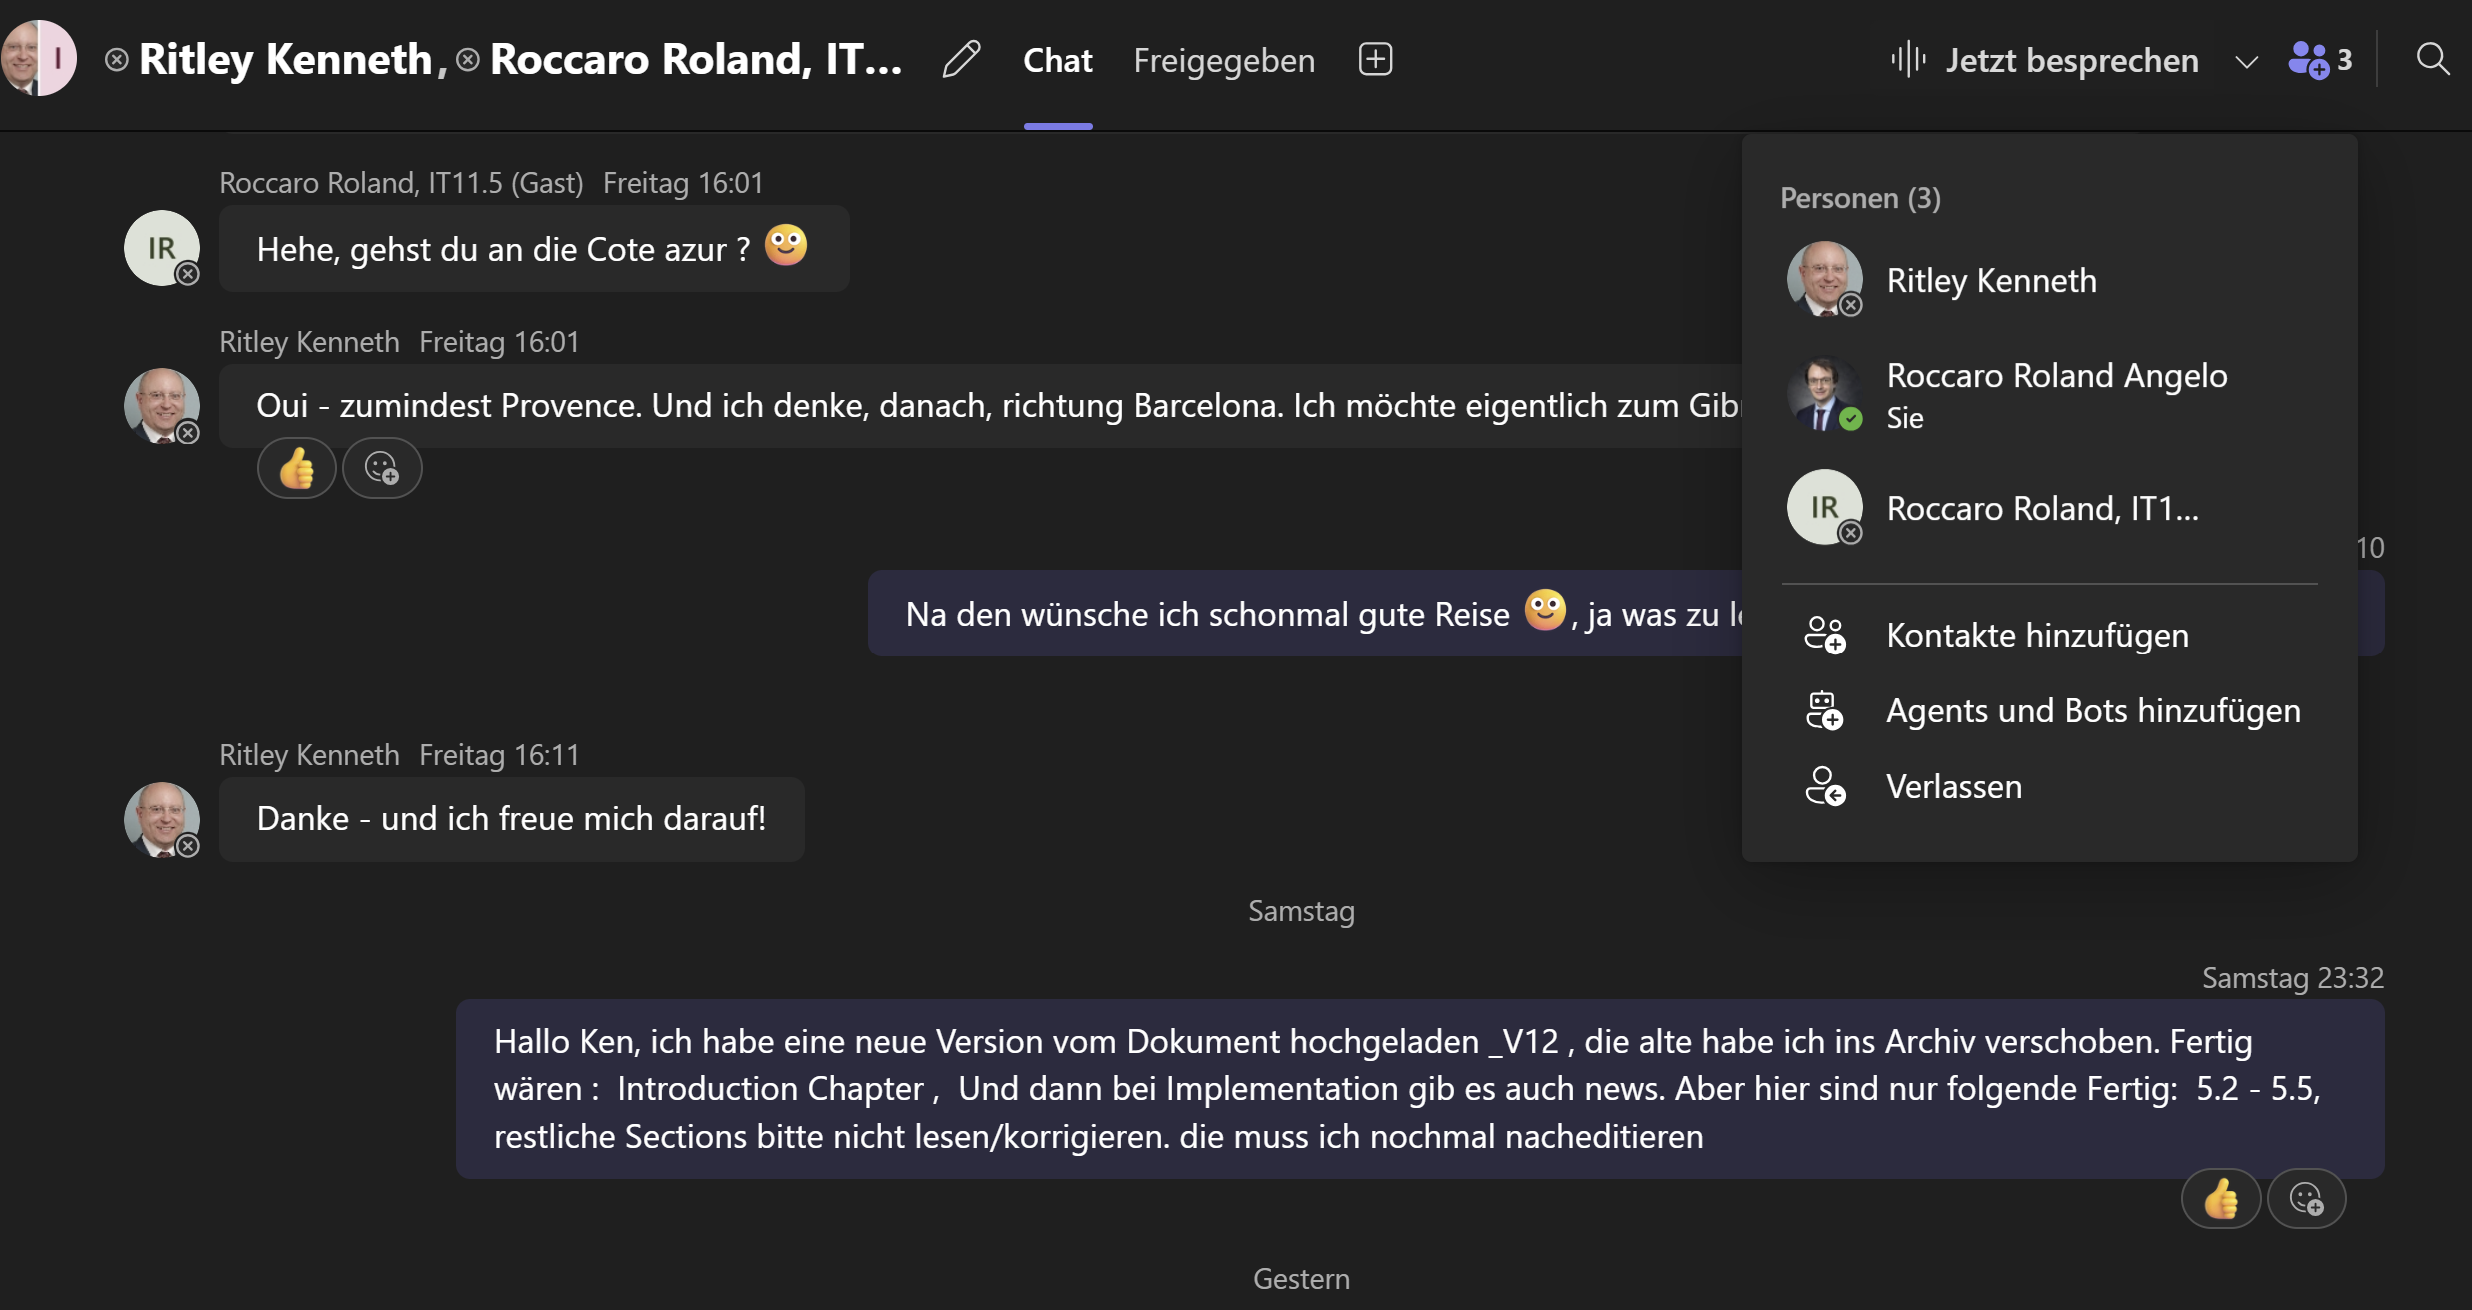
\includegraphics[width=0.8\textwidth]{./content/img/ProjectManagement/ProjMgmt_Teams_Chat.png}
    \caption{Shared chat using Teams}
    \label{fig:teams_shared_chat}
\end{figure}

A second important application of MS Teams is a document management system. This includes source documents, document versions, and related materials. All relevant documents are stored within this structure, which is designed to grow as needed.

\begin{figure}[H]
    \centering
    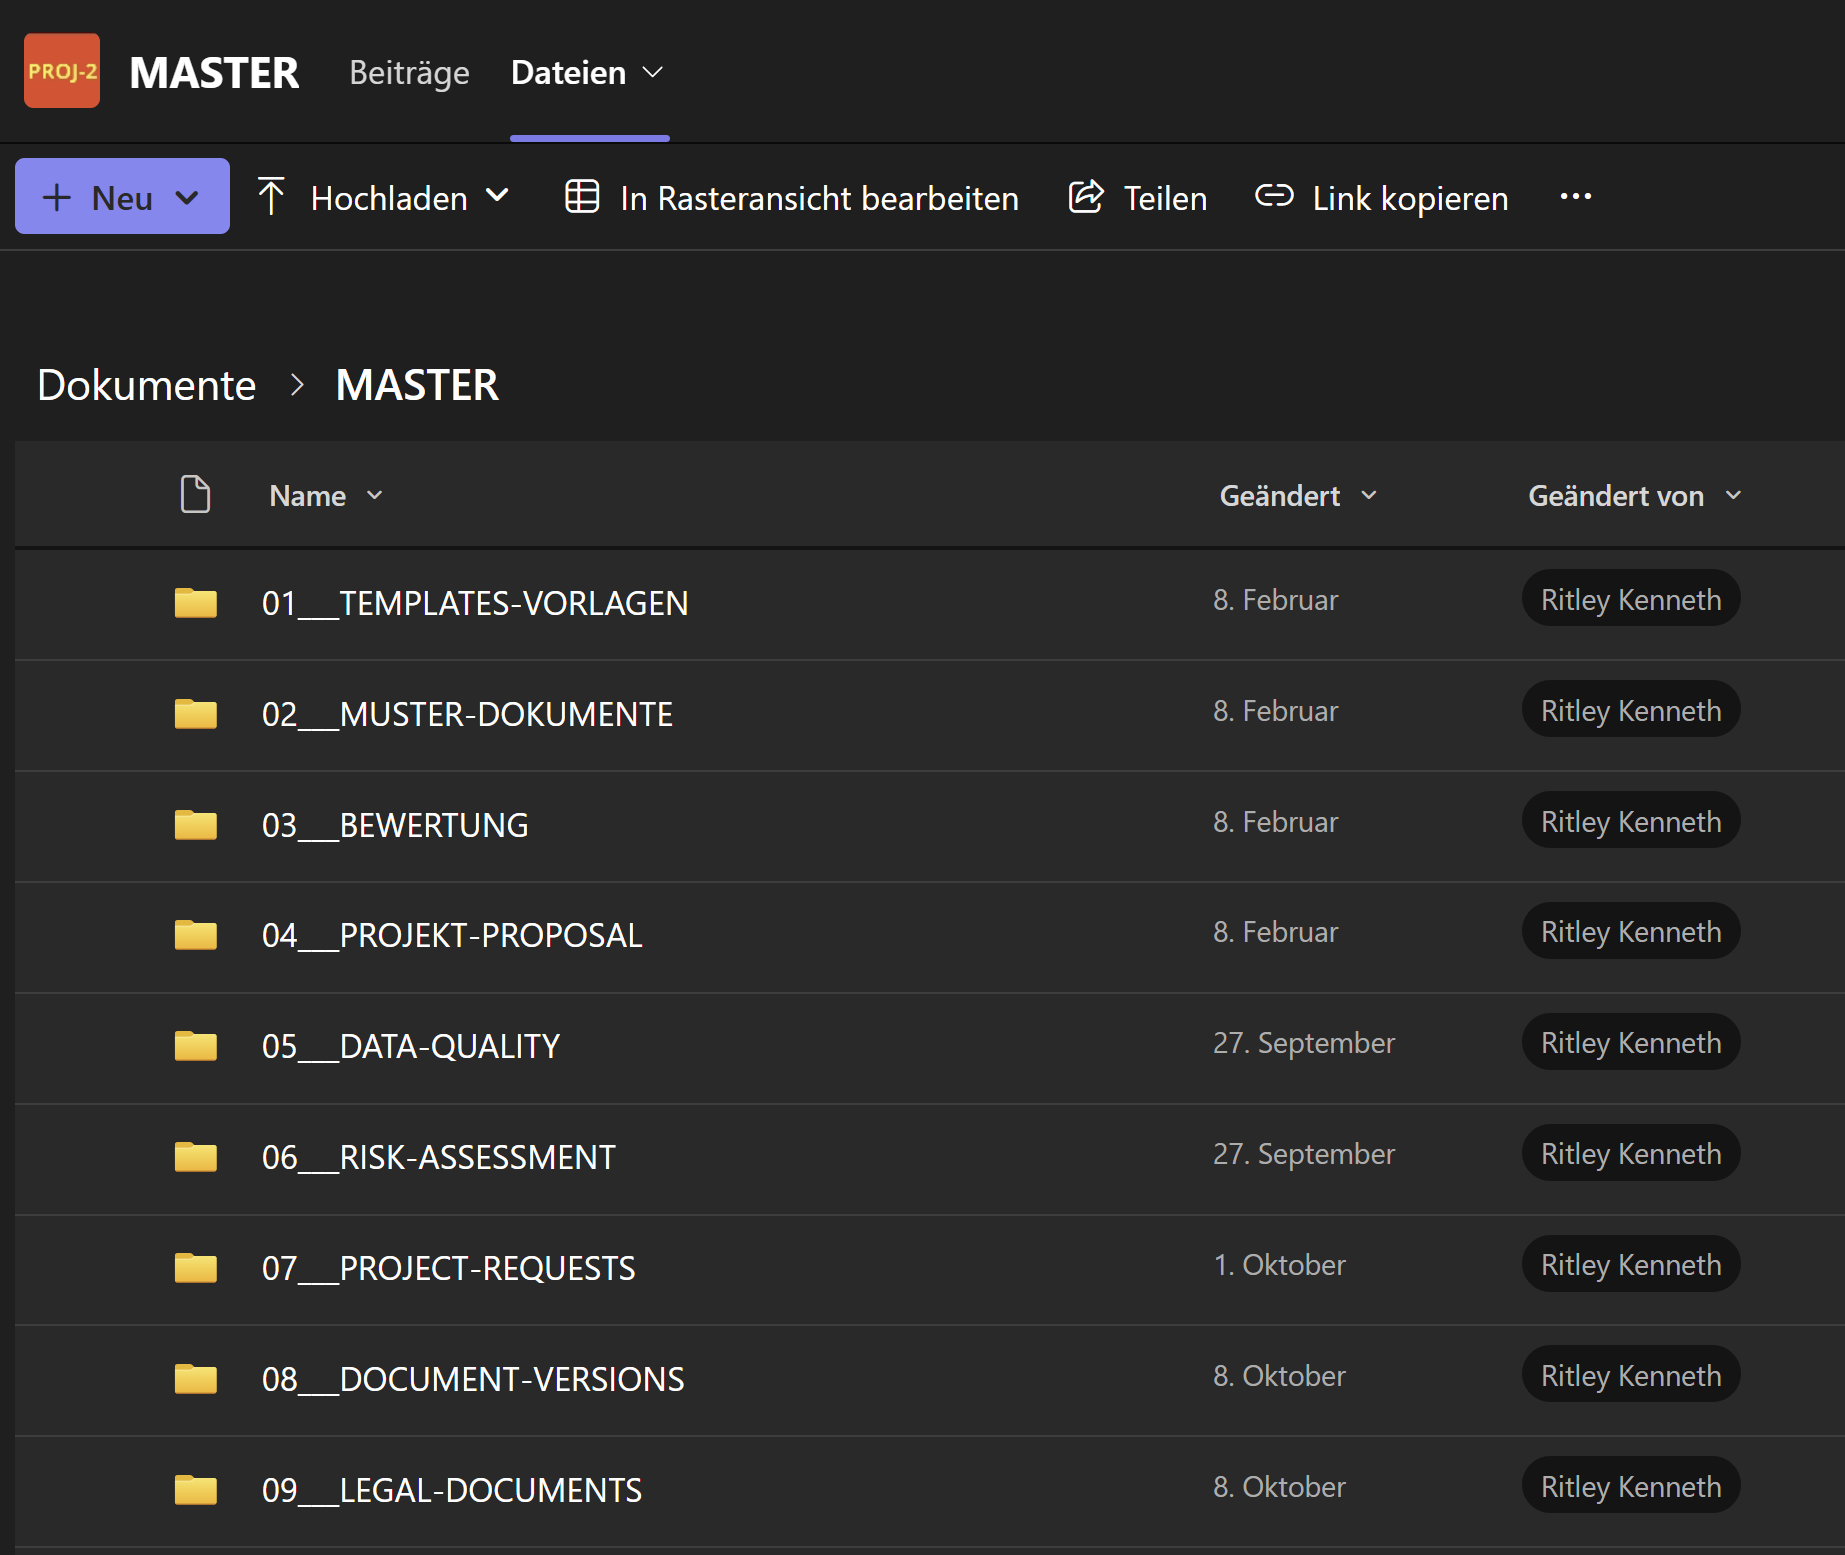
\includegraphics[width=0.8\textwidth]{./content/img/ProjectManagement/ProjMgmt_Teams_Documents.png}
    \caption{Project document store used with Teams}
    \label{fig:teams_document_store}
\end{figure}

\subsection*{LaTeX}
LaTeX was the tool chosen for the main writing process by the academic team. The primary reason for selecting this tool was the consistency of the document structure. It allows changes to be made in a large document without the document becoming unstable. The tool was specifically selected for this higher consistency compared to Word. The fact that the creation of some stylistic elements takes more time than with a \gls{WYSIWYG} editor such as Word was accepted, particularly as design was valued lower than document content. Finally, the consistency of being able to reference text sections within the document and the ability to automatically generate lists of figures and tables were seen as additional benefits. Furthermore, the automatic glossary and citation features using Biber were considered advantages for which the slower writing process without a WYSIWYG editor was accepted. Due to the learning effort involved in using \LaTeX, the following badge was earned during the course of the research.

\begin{figure}[H]
    \centering
    
\includegraphics[width=0.65\textwidth]{./content/img/ProjectManagement/RolandMasterOfLatex.png}
    \caption{Humorous illustration symbolising the extensive use of \LaTeX\ throughout the preparation of this report and the associated learning experience during the project.}
    \label{fig:latex_mastery}
\end{figure}

\subsection*{GitHub}
For maintaining version control of any created artefacts, the public GitHub was used with the private account of the academic team. It was mainly used as a repository. This Git distribution was chosen because it is free to use and already well known to the team, with all required accounts in place, so no additional adoption or learning effort was required before starting. GitHub was not only used to store the document and track its progress, but also to manage all required sources such as tables and images used in the document.

For the writing process, the use of GitHub as a backup mechanism was particularly important. As all sources are stored in GitHub, the project was safeguarded against hardware failures of the working device, which is one risk mitigation measure. Continuously committing and pushing changes made the progress of the writing process traceable and supported the iterative writing approach which was chosen. This proved useful when the document PDF could no longer be generated, as the last version that compiled without errors could be identified. Finally, storing the sources on GitHub allowed access from different devices, which was useful when transferring materials such as screenshots from the work device to the study device.

\subsection*{ChatGPT}
LLMs are now an indispensable part of work. To note how ChatGPT was used in this project, it was given the following prompt:
\begin{quote}
Hi ChatGPT, please look at the other chats I have with you and tell me in which ways you supported me during my academic project over the past months since September 2025. Please create a subsection for my scientific work which I can reference.
\end{quote}

The following subsection was completely AI generated content by ChatGPT, without further editing.
{\itshape
\subsubsection*{ChatGPT}

To document the support provided by ChatGPT, a summary of the assistance received during the academic project was generated directly by the tool itself:
The request asked ChatGPT to review prior interactions and describe the ways in which it supported the academic project over the past months since September 2025. The resulting subsection is intended for inclusion in the scientific work and can be referenced accordingly \cite{chatgpt_ai_assistance_2025}.



The following subsection is entirely AI-generated content produced by ChatGPT, without further editing  \cite{chatgpt_ai_assistance_2025}.

\subsubsection*{Use of AI Assistance in the Research Process}
\label{sec:use_of_genai}

During the preparation and initial phases of this Master Thesis, starting in August 2026, OpenAI's ChatGPT was used as a supporting tool for academic writing, project organisation, methodological discussions, and document preparation.

The use of ChatGPT can be divided into several areas:

\begin{itemize}
    \item \textbf{Academic writing and proofreading:}
    ChatGPT was used to review English texts for spelling, grammar, readability, and academic style. It also suggested alternative formulations, improved transitions between paragraphs, and helped identify unclear or insufficiently supported statements. The author reviewed and selected the proposed changes.

    \item \textbf{Thesis structure and research planning:}
    ChatGPT supported discussions concerning the organisation of the thesis, the formulation of research objectives and questions, and the distinction between previous academic projects and the new contributions of the Master Thesis. It was also used to critically discuss the scope of the work and possible approaches to scientific evaluation.

    \item \textbf{Research methodology and scientific reasoning:}
    ChatGPT was used as a discussion partner to explore possible research approaches, evaluation criteria, and methodological considerations. Its suggestions served as input for further examination rather than as independently verified scientific findings.

    \item \textbf{Project management and organisation:}
    ChatGPT assisted in preparing project plans, structuring activities, defining milestones, and developing an Excel-based semester planning tool. It also supported the organisation of separate discussion topics for different aspects of the thesis.

    \item \textbf{\LaTeX{} and document preparation:}
    ChatGPT provided assistance with \LaTeX{} syntax, document structure, figure captions, references, formatting, and troubleshooting. It was also used to convert and adapt existing text into \LaTeX{}-compatible formats.

    \item \textbf{Review of existing academic work:}
    ChatGPT supported the examination and comparison of material from the two preceding academic projects. Particular attention was given to identifying which results constituted previous work and which activities would need to provide a new scientific or technical contribution.
\end{itemize}

ChatGPT was used as an assistive tool rather than as an independent source of scientific evidence. The responsibility for research decisions, technical implementation, verification of information, interpretation of results, and the final content of the thesis remained with the author. AI-generated suggestions were subject to review and were not considered substitutes for academic literature, empirical evidence, or expert feedback.
}
\section{Milestones, TODO}
\label{ProjMgmtMilestones}

Todo,
Work for Future Roland
He will have to describe the milestones

 

The following phase are defining blocks which can be closed after completing each and move on. The conclusion and start of each phase are used to review and adapt the current state.
The milestones are events during the course of the phases. Each milestone will be documented if it has been reached in time. Furthermore, any adaptions required to the milestone plans have to be documented.


The milestone timelines are setup as follows before project start.

\begin{itemize}
    \item Milestone 1, use case defined: 18.10.2026
    \item Milestone 2, Stakeholder meetings held: 15.11.2026
    \item Milestone 3, Error documentation by stakeholders started: 29.11.2026
    \item Milestone 4, Development environment set, initial setup of tools: 13.12.2026
    \item Milestone 5, MVP has been setup: 21.03.2027
    \item Milestone 6, MVP presented to Post stakeholders: 04.04.2027
    \item Milestone 7, Outline of second iteration defined: 18.04.2027
    \item Milestone 8, Data of different approaches compared: 16.05.2027
    \item Milestone 9, Thesis document completed: 11.07.2027
    \item Milestone 10, Presentation ready: 25.07.2027
\end{itemize}

\begin{figure}[H]
    \centering
    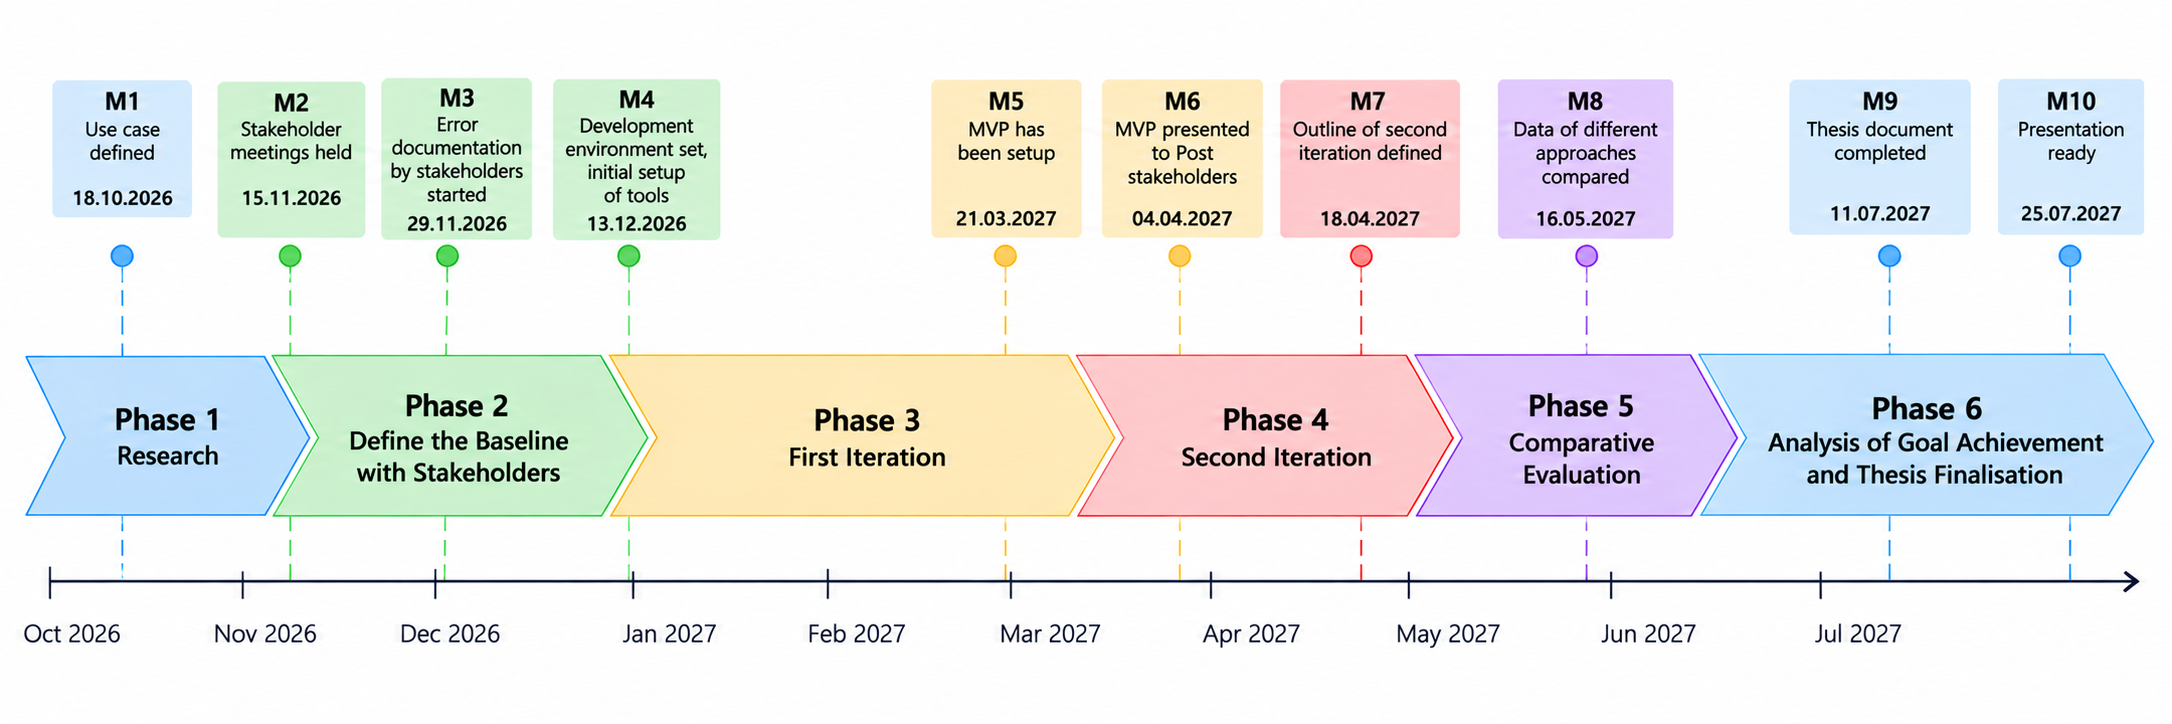
\includegraphics[width=0.8\textwidth]{./content/img/Mth/ProjectManagement/MilestoneTimelineAdapted_2.png}
    \caption{Milestones and phases defined at the start of the project}
    \label{fig:projmgmt_milestones_and_phases}
\end{figure}




\section{Effort planning and review, TODO}

Effort planning and review are carried out to plan and confirm the time allocated to each phase. Additionally, this provides confirmation of the effort structure. Furthermore, it establishes the framework for a later review of the planned hours.



\subsection*{Effort planning}

The effort was planned according to the duration of the phases. These were laid out in the previous section and provide a start and end time for each phase. Thus, each phase contains a defined number of weeks. The planned effort is therefore first measured as an absolute number of weeks. Using this count, a relative effort is obtained by comparing the number of weeks per phase with the total number of weeks planned. Which results in the following formula to get the relative time allocation per phase. 

\[
\text{Relative time allocation}_i =
\frac{\text{Weeks allocated to phase } i}
{\text{Total planned weeks}} \times 100\%
\]



In the upcoming table, the relevant data for the calculation of the phase efforts is detailed. Phases always end according to the two-week sprint rhythm but do not necessarily end with the phase's last milestone. The table shows the following information:

\begin{itemize}
    \item \textbf{Phase:} The number of the phase for each line
    \item \textbf{Milestone:} This is either the milestone number or "end" in case it is the end of a phase.
    \item \textbf{MS date:} The date of the milestone or phase end date
    \item \textbf{Name of milestone:} The abbreviated name of the milestone or the end of a phase
    \item \textbf{Phase weeks total:} The total number of weeks spent in that phase
    \item \textbf{Relative percent:} According to the above formula, what percentage of the total time is spent in this phase.
\end{itemize}

\begin{table}[htbp]
    \centering
    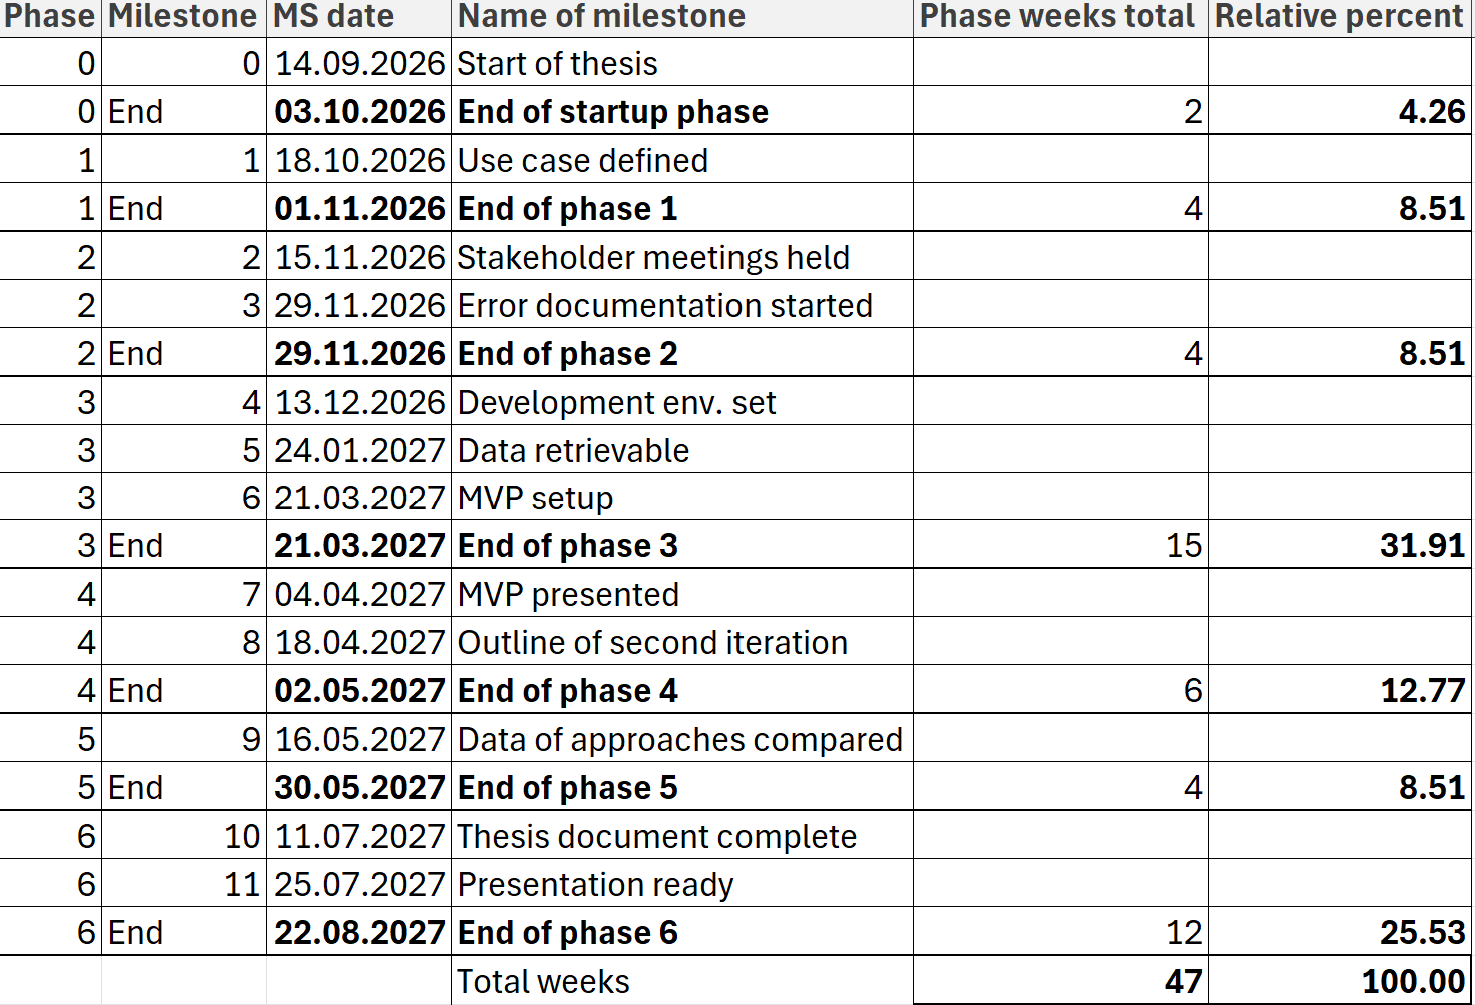
\includegraphics[width=\textwidth]{./content/img/Mth/ProjectManagement/TimeLinePercentage.png}
    \caption{Distribution of planned project duration across project phases}
    \label{tab:timeline_percentage}
\end{table}




\subsection*{Two ways of recorded time}
First to some rules as to how time can be registered. Regarding work efforts its important to note that the academic team has an agreement with Swiss Post defining which efforts are considered work time and which not. 
As per agreement, the research part and the writing part of this document are not to be noted as work time, however the remainder of activities such as implementation, documenting work state in Jira or confluence etc. are considered work efforts and are noted into the time tracking at swiss post as such. 

This agreement leads to two different ways of tracking time. At Swiss Post, time is tracked directly with their SAP time-tracking \gls{MIAR} system, where the efforts are recorded against a specific project account. This makes it easy to export and track them for monitoring purposes in the thesis.

Second, academic efforts committed to the project outside the agreement were recorded separately. The work was then registered in blocks of continuous work on project-related tasks, including short breaks. However, longer breaks, such as lunch, resulted in a new block being created.


\subsection*{Planning review}
At the end of the thesis, the number of hours tracked is summed up per phase, based on the start and end dates that were actually reached, taking into account any deviations. These totals per phase and the overall total lead to a second relative measure. The two relative measures per phase are then compared and evaluated. A summary of this is provided along with the analysis of the planning process at the end of this project management chapter.

\section{Risk management}
\label{ProjMgmtRisk}


In this section, the approach taken to risk management is described. Risk management is essential to the success of any project, as it enables planning for and potentially preventing dangers that may occur during its course. When such risks are not handled, they can endanger the progress of the project. The risk management process consists of several steps \cite{RiskmgmtWikipedia}. First, the risks are identified and classified as to their nature. Next, they are weighted according to how they might impact this project; this includes a consideration of the probability that the risks may arise, and the level of damage that may occur. After this, the specific handling of each risk is defined; these are the concrete measures that are taken to lower how the risk may impact the project. Finally, ongoing monitoring and review of the risks is carried out on a regular basis throughout the project.

\subsection*{Risk identification and classification}

The identification of risks has been carried out for this project, following an extensive brainstorming approach. Each risk has been grouped into a category (e.g. goal, time and organization, etc.), and each risk has been classified according to the likelihood of is occurance and severity it would cause to the project. Both criteria are evaluated based on the project team’s \gls{riskappetite} and ranked according to the following definitions.

\begin{itemize}
    \item \textbf{Likelihood:} What is the expected likelihood of a risk coming into effect
    \begin{itemize}
        \item \textbf{1} Rare
        \item \textbf{2} Unlikely
        \item \textbf{3} Possible
        \item \textbf{4} Likely
        \item \textbf{5} Almost Certain
    \end{itemize}

    \item \textbf{Severity:} How severe are the consequences of the risk coming into effect
    \begin{itemize}
        \item \textbf{1} Insignificant
        \item \textbf{2} Minor
        \item \textbf{3} Moderate
        \item \textbf{4} Major
        \item \textbf{5} Severe
    \end{itemize}
\end{itemize}



The identified  risks, along with their likelihood and severity, are listed in Table \ref{tab:risks}.

\begin{longtable}{@{} C{1.1cm} L{3.2cm} L{8.1cm} C{1.6cm} C{1.6cm} @{}}
\caption{Project Risk Overview}\label{tab:risks}\\


\toprule
\textbf{No.} & \textbf{Group} & \textbf{Risk} & \textbf{Likelihood} & \textbf{Severity} \\
\midrule
\endfirsthead

\toprule
\textbf{No.} & \textbf{Group} & \textbf{Risk} & \textbf{Likelihood} & \textbf{Severity} \\
\midrule
\endhead

\midrule
\multicolumn{5}{r}{\small Continued on next page} \\
\endfoot

\bottomrule
\endlastfoot

1 & Goal & Unclear question & 2 & 2 \\
2 & Goal & Unclear goals & 2 & 3 \\
3 & Time and Organisation & Insufficient expertise & 4 & 2 \\
4 & Time and Organisation & Underestimated time/effort & 4 & 4 \\
5 & Time and Organisation & Other study projects & 3 & 3 \\
6 & Time and Organisation & Work projects & 4 & 3 \\
7 & Time and Organisation & Procrastination & 3 & 2 \\
8 & Human Resources & Unavailability of main project staff, e.g. due to illness & 5 & 4 \\
9 & Human Resources & Unavailability of advisor, e.g. due to illness or accident & 3 & 3 \\
10 & Tech and Infrastructure & Software version/library/dependency & 4 & 3 \\
11 & Tech and Infrastructure & Hardware is damaged & 2 & 4 \\
12 & Data and Research & Data related & 4 & 4 \\
13 & Data and Research & Non-reproducible work & 1 & 5 \\
14 & Ethical and Legal & Plagiarism or incorrect citation & 2 & 5 \\
15 & Ethical and Legal & Copyright & 1 & 5 \\
16 & Communication and Cooperation & Bad communication with stakeholders or advisor & 1 & 4 \\
17 & Communication and Cooperation & Insufficient exchange with external partners & 3 & 5 \\
18 & Force Majeure & Unforeseen family crisis & 2 & 5 \\
19 & Force Majeure & General force majeure & 1 & 5 \\
20 & Unknown Process & The required management process is unknown & 4 & 2 \\
21 & Communication and Cooperation & Required resources are not available when needed, or responsibilities are unclear & 3 & 4 \\
22 & Organisational & Changes pushed by the organisation & 3 & 4 \\
23 & Data and Research & Insufficient scientific contribution & 1 & 5 \\

\end{longtable}


\subsection*{Risk heat map}
After carrying out the initial identification and classification, it is not always easy to determine which risks require the most attention. To support this task, a Risk Heat Map is used, in which each risk is plotted in a two-dimensional matrix according to its likelihood and severity. This visualisation highlights the risks that pose the greatest threat to the project and should be considered for priority treatment. The colours in the Risk Heat Map \ref{tab:risks_sev_likely} correspond to these descriptions. 


\begin{itemize}
    \item \textbf{Green} Low
    \item \textbf{Yellow} Medium
    \item \textbf{Orange} High
    \item \textbf{Red} Very High
\end{itemize}



The previous table results in the following heat map, which allows the reader to more easily grasp which items are considered more dangerous to the project. It shows that four risks are classified as red and therefore require special attention. How these risks, as well as the others, are addressed is described in the following section.



\begin{table}[H]
    \centering
    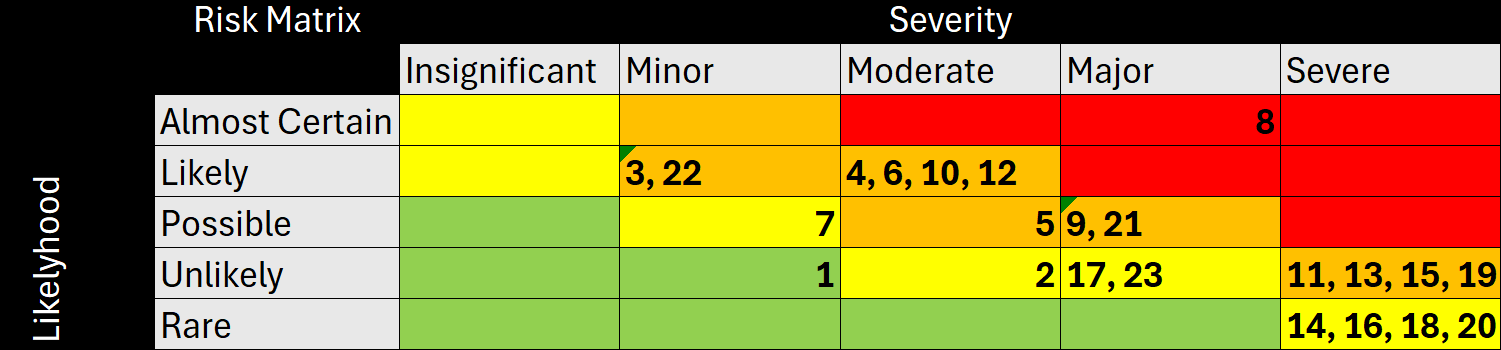
\includegraphics[width=0.95\textwidth]{./content/img/Mth/ProjectManagement/Risks_Mth_Initial.png}
    \caption{Initial risk assessment at the beginning of the Master Thesis.}
    \label{tab:mth_initial_risk_assessment}
\end{table}



\subsubsection*{Previous heat map}
As a reference for the continued risk management over the course of the entire initiative, the following heat map shows the status at the beginning of the second project. This illustrates that, over the course of the initiative, risks have been added and are now evaluated differently by the project team.

\begin{table}[H]
    \centering
    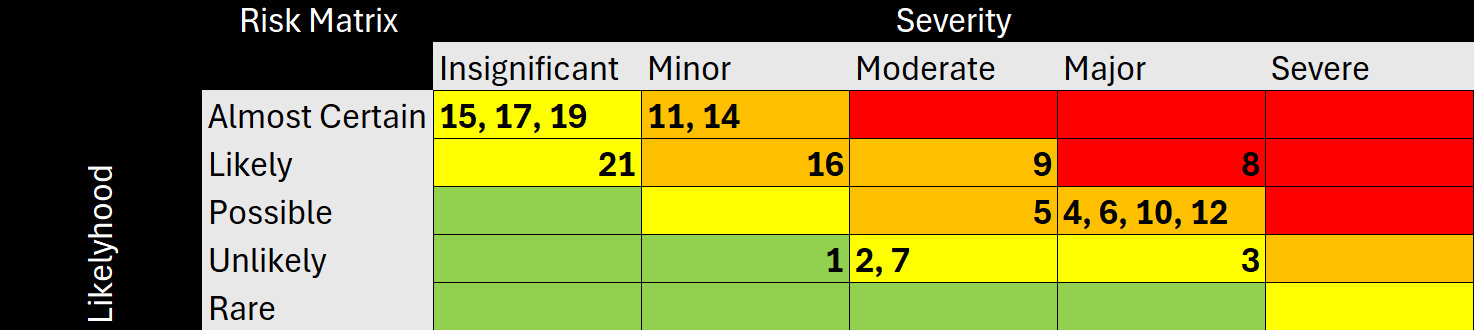
\includegraphics[width=0.95\textwidth]{./content/img/Mth/ProjectManagement/Risks_Mth_Project1.png}
    \caption{Risk matrix from Project 1.}
    \label{tab:risks_sev_likely}
\end{table}



\subsection*{Risk strategies and mitigation strategies}

Risk strategies are the high level approaches to dealing with the risks, and the risk mitigations are the concrete plans developed to manage identified risks. In the following table, an overview of the individual risks is provided, including their selected treatment and a brief justification. Naturally, it is neither practical nor feasible to completely eliminate every risk; therefore, based on likelihood and severity, as well as the team’s \gls{riskappetite}, each risk was assigned one of the following strategies:

\begin{itemize}
\item \textbf{Accept} – the risk and its potential impact are acknowledged, but no measures are taken
\item \textbf{Reduce} – the risk is mitigated by applying additional measures to lower its impact or probability
\item \textbf{Transfer} – the responsibility for handling the risk is assigned to another party
\item \textbf{Avoid} – the project is adapted in a way that prevents the risk from materialising
\end{itemize}

\begin{longtable}{@{} C{1.2cm} L{2.5cm} L{4.5cm} L{2.5cm} L{5cm} @{}}
\caption{Risk Strategy and Treatment Plan}\label{tab:risk_treatment}\\

\toprule
\textbf{No.} & \textbf{Risk} & \textbf{Risk Description} & \textbf{Treatment} & \textbf{Treatment Description} \\
\midrule
\endfirsthead

\toprule
\textbf{No.} & \textbf{Risk} & \textbf{Risk Description} & \textbf{Treatment} & \textbf{Treatment Description} \\
\midrule
\endhead

\midrule
\multicolumn{5}{r}{\small Continued on next page} \\
\endfoot

\bottomrule
\endlastfoot


1 & Goal & Unclear question & Reduce & Define SMART goals. \\
2 & Goal & Unclear goals & Reduce & Describe which goals are within the scope. \\
3 & Time and Organisation & Insufficient expertise & Accept & Learning is part of the process, but additional time needs to be planned. \\
4 & Time and Organisation & Underestimated time/effort & Reduce & Phases and milestones are set up as progress checks. \\
5 & Time and Organisation & Other study projects & Accept & Use minimal time for other projects/classes. \\
6 & Time and Organisation & Work projects & Reduce & Reduce the risk by starting early and defining blockers for study work. \\
7 & Time and Organisation & Procrastination & Reduce & Start early. \\
8 & Human Resources & Unavailability of main project staff, e.g. due to illness & Reduce & This happened before the start. Provide the contact details of the partner working at BFH and document the situation in case it happens again. \\
9 & Human Resources & Unavailability of advisor, e.g. due to illness or accident & Transfer & The advisor should define an emergency replacement. \\
10 & Tech and Infrastructure & Software version/library/dependency & Accept & Run the code multiple times and use test cases, e.g. unit tests. \\
11 & Tech and Infrastructure & Hardware is damaged & Reduce & Second laptop; code and documentation on GitHub, Miro, Teams, and Outlook. \\
12 & Data and Research & Data related & Accept & No preparation is planned. \\
13 & Data and Research & Not reproducible work & Reduce & Document major steps, upload versions of the document to GitHub, and use Kanban in Miro to document tasks. \\
14 & Ethical and Legal & Plagiarism or incorrect citation & Reduce & Use citations and a bibliography. \\
15 & Ethical and Legal & Copyright & Accept & Declare sources in the bibliography. For Swiss Post sources, use only public documents. \\
16 & Communication and Cooperation & Bad communication with stakeholders or advisor & Reduce & Weekly advisor meetings (Jour Fixe). \\
17 & Communication and Cooperation & Insufficient exchange with external partners & Reduce & Include stakeholders in the Scrum team. \\
18 & Force Majeure & Unforeseen family crisis & Accept & Document it in the Miro calendar if it happens. \\
19 & Force Majeure & General force majeure & Accept & Document it in the Miro calendar if it happens. \\
20 & Unknown Process & The required management process is unknown & Reduce & Projects 1 and 2 established many of the required steps. However, it is still likely that something new may arise. \\
21 & Communication and Cooperation & Required resources are not available when needed, or responsibilities are unclear & Reduce & Schedule calls early and search for external resources before starting work blocks. \\
22 & Organisational & Changes pushed by the organisation & Accept & Change is constant; discussions with teams are required. \\
23 & Data and Research & Insufficient scientific contribution & Reduce & Provide continuous feedback and hold weekly calls to identify missing contributions early. \\

\end{longtable}

\subsection*{Implementation of risk mitigation strategies}
Identifying the key risks is the first step in the overall risk management approach; this is followed by defining measures for each of the risks. In the following table, the implementation of these measures is documented. The measures have been implemented according to the strategies and descriptions outlined above. Table \ref{tab:risk_actions} provides an overview of the actions taken and when they were carried out.


\begin{longtable}{@{}C{1cm}L{3.5cm}L{9cm}C{2.5cm}@{}}
\caption{Risk Strategy and Action Overview}\label{tab:risk_actions}\\

\toprule
\textbf{No.} & \textbf{Risk} & \textbf{Strategy Decision / What} & \textbf{When} \\
\midrule
\endfirsthead

\multicolumn{4}{c}{\bfseries \tablename\ \thetable{} -- continued from previous page} \\
\toprule
\textbf{No.} & \textbf{Risk} & \textbf{Strategy Decision / What} & \textbf{When} \\
\midrule
\endhead

\midrule
\multicolumn{4}{r}{\small Continued on next page} \\
\bottomrule
\endfoot

\bottomrule
\endlastfoot


1 & Unclear question & Reduce: SMART goals have been defined in the research section. & 24.10.2026 \\
2 & Unclear goals & Reduce: The introduction describes which parts of the initial project description are included in this document. & 24.10.2026 \\
3 & Insufficient expertise & Accept: Nothing done. & 24.10.2026 \\
4 & Underestimated time/effort & Reduce: Phases and milestones are set up as progress checks. & 24.10.2026 \\
5 & Other study projects & Accept: Nothing done. & 24.10.2026 \\
6 & Work projects & Reduce: Discussed availability with the other team, added blockers to the work calendar, invited the work account to the Jour Fixe meeting series, set weekend blockers in the study account, and researched optimal or minimal study plans with ChatGPT. & 24.10.2026 \\
7 & Procrastination & Reduce: Work on the project started on 14.09.2026, with the first meeting with the expert in the same week. & 24.10.2026 \\
8 & Unavailability of main project staff, e.g. due to illness & Reduce: The partner's contact details were provided in Teams and added to the Miro board. & 24.10.2026 \\
9 & Unavailability of advisor, e.g. due to illness or accident & Transfer: Asked for a contact; Jürgen Vogel was confirmed as the replacement. & 24.10.2026 \\
10 & Software version/library/dependency & Accept: Nothing done. & 24.10.2026 \\
11 & Hardware is damaged & A second laptop is available at home. The LaTeX document is a GitHub project, and documentation is stored in Miro. The work laptop can also be used for most tasks but does not have LaTeX installed. & 24.10.2026 \\
12 & Data related & Accept: Nothing done. & 24.10.2026 \\
13 & Not reproducible work & Reduce: GitHub project for the LaTeX document. & 24.10.2026 \\
14 & Plagiarism or incorrect citation & Reduce: JabRef is used as a GUI for the bibliography, and Biber is used for compilation. & 24.10.2026 \\
15 & Copyright & Accept: Nothing done. & 24.10.2026 \\
16 & Bad communication with stakeholders or advisor & Reduce: Jour Fixe has been set up. & 24.10.2026 \\
17 & Insufficient exchange with external partners & Reduce: Maintain communication channels even when changing teams. & 24.10.2026 \\
18 & Unforeseen family crisis & Accept: Nothing done. & 24.10.2026 \\
19 & General force majeure & Accept: Nothing done. & 24.10.2026 \\
20 & The required management process is unknown & Reduce: It is still important to address new requirements as soon as they appear. & 24.10.2026 \\
21 & Required resources are not available when needed, or responsibilities are unclear & Reduce: Search for external resources before starting your own work. & 24.10.2026 \\
22 & Changes pushed by the organisation & Accept: Exchange information with teams. & 24.10.2026 \\
23 & Insufficient scientific contribution & Reduce: Addressed as part of the Jour Fixe. & 24.10.2026 \\

\end{longtable}

\subsection*{Ongoing risk monitoring}
A critical step in the risk management process is ongoing monitoring. Monitoring the risks ensures that the defined measures remain valid and that any risks that may materialise are identified. If a new risk is identified or causes a disruption to the project, it will be documented. Additionally, an appropriate measure to handle its impact will be defined. Monitoring of the risks will be performed every second Friday of each month. Detailed information about the risk monitoring process is provided in the appendix \ref{RiskMonitoring}.
These risk check-ins will contain the following information:

\begin{itemize}
\item Number of risk: same as in the tables above
\item Name of risk: same as in the tables above
\item Occurred: did the risk occur (yes or no)?
\item Details: what happened?
\item Cause: brief analysis of why it happened
\item Measures taken: what measures have been taken?
\item Measure date: on what date were measures taken?
\end{itemize}

\subsection*{Risk review at project completion}

Finally, a review of the risks will be held at the end of the project. This will address which risks came into effect and which did not. Additionally, changes to the perception of the risks will be documented at the start of the master thesis. 

\section{Execution and review, TODO}


Todo,
Work for Future Roland
He will have to describe the How well project management did work out...
e.g. Phases
Milestones
Tools...
Risks...

\subsection*{Project plan and work packages, TODO}
Todo,
Work for Future Roland
He will have to describe the project plan and the planned workpackages
See at following content to take the needed out of this


